\documentclass[11pt]{article}

\usepackage{a4wide}
\usepackage{authblk}
\usepackage{amsmath,amssymb}
\usepackage{amsthm}
\usepackage[dvipdfmx]{graphicx}
\usepackage{here}
\usepackage{url}

\setlength{\topmargin}{-10mm}

\pdfinclusionerrorlevel=1
\pdfminorversion=7

\pdfoutput=1

\usepackage{thmtools}

\newtheorem{theorem}{Theorem}
\newtheorem{lemma}{Lemma}
\newtheorem{corollary}{Corollary}

\theoremstyle{definition}
\newtheorem{definition}{Definition}
\newtheorem{problem}{Problem}
\newtheorem{remark}{Remark}
\newtheorem{example}{Example}
\newtheorem*{claim}{Claim}

%\renewenvironment{proof}{\begin{trivlist} \item{\textit{Proof.}}}{\end{trivlist}}

\usepackage[final,mode=multiuser]{fixme}
%\usepackage[draft,mode=multiuser]{fixme}
\fxsetup{theme=color}
\definecolor{fxtarget}{rgb}{0.0000,0.0000,0.7000}
\fxuseenvlayout{colorsig}
\fxusetargetlayout{color}
\FXRegisterAuthor{rh}{ahr}{RH}
\FXRegisterAuthor{hf}{ahf}{HF}
\FXRegisterAuthor{si}{asi}{SI}
\fxsetface{env}{}

%%%%%%%%%%%%%%%%%%%%%%%%%%%%%%%%%%%%%%%%%%%%%%%%%%%

\newcommand{\Prefix}{\mathsf{Prefix}}
\newcommand{\Substr}{\mathsf{Substr}}
\newcommand{\Suffix}{\mathsf{Suffix}}
\newcommand{\occ}{\mathsf{occ}}
\newcommand{\Long}{\mathsf{long}}
\newcommand{\CDAWG}{\mathsf{CDAWG}}

\newcommand{\lrep}{\mathsf{lexp}}
\newcommand{\rrep}{\mathsf{rexp}}

%\newcommand{\lext}[2]{\overset{#2}{\overleftarrow{#1}}}
%\newcommand{\lext}[2]{\overset{#2}{\overrightarrow{#1}}}

\newcommand{\EqrL}{\equiv^{\mathrm{L}}}
\newcommand{\EqrR}{\equiv^{\mathrm{R}}}
\newcommand{\EqcL}[1]{[{#1}]^{\mathrm{L}}}
\newcommand{\EqcR}[1]{[{#1}]^{\mathrm{R}}}
\newcommand{\EqcB}[1]{[{#1}]}

\newcommand{\LeftM}{\mathsf{LeftM}}
\newcommand{\RightM}{\mathsf{RightM}}
\newcommand{\M}{\mathsf{M}}
\newcommand{\D}{\mathsf{d}}

\newcommand{\size}{\mathsf{e}}

\newcommand{\MSIns}{\mathsf{MS}_{\mathrm{Ins}}}
\newcommand{\MSDel}{\mathsf{MS}_{\mathrm{Del}}}
\newcommand{\MSSub}{\mathsf{MS}_{\mathrm{Sub}}}

\newcommand{\N}{\mathsf{N}}
\newcommand{\None}{\mathsf{N}_{\mathrm{1}}}
\newcommand{\Ntwo}{\mathsf{N}_{\mathrm{2}}}
\newcommand{\Nthree}{\mathsf{N}_{\mathrm{3}}}
\newcommand{\Nv}{\mathsf{N}_{\mathrm{3B}}}
\newcommand{\Q}{\mathsf{Q}}
\newcommand{\Qn}{\mathsf{Q}_{\mathrm{1}}}
\newcommand{\Qnotn}{\mathsf{Q}_{\mathrm{2}}}
\newcommand{\Nnotv}{\mathsf{N}_{\mathrm{3A}}}

\newcommand{\ed}{\mathsf{ed}}

\newcommand{\polylog}{\mathrm{polylog}}

%%%%%%%%%%%%%%%%%%%%%%%%%%%%%%%%%%%%%%%%%%%%%%%%%%%


\begin{document}

\title{Constant sensitivity on the CDAWGs}

\author[1]{Rikuya~Hamai}
\author[1]{Hiroto~Fujimaru}
\author[2]{Shunsuke~Inenaga}

\affil[1]{Department of Information Science and Technology, Kyushu University, Japan}
\affil[2]{Department of Informatics, Kyushu University, Japan}

\date{}
\maketitle

\begin{abstract}
\emph{Compact directed acyclic word graphs} (\emph{CDAWGs}) [Blumer et al. 1987] are a fundamental data structure on strings with applications in text pattern searching, data compression, and pattern discovery. Intuitively, the CDAWG of a string $T$ is obtained by merging isomorphic subtrees of the suffix tree [Weiner 1973] of the same string $T$, and thus CDAWGs are a compact indexing structure. In this paper, we investigate the sensitivity of CDAWGs when a single character edit operation is performed at an arbitrary position in $T$.
We show that the size of the CDAWG after an edit operation on $T$
is asymptotically at most 8 times larger than the original CDAWG before the edit.
\end{abstract}

\section{Introduction}
\label{sec:introduction}
The business processes of organizations are experiencing ever-increasing complexity due to the large amount of data, high number of users, and high-tech devices involved \cite{martin2021pmopportunitieschallenges, beerepoot2023biggestbpmproblems}. This complexity may cause business processes to deviate from normal control flow due to unforeseen and disruptive anomalies \cite{adams2023proceddsriftdetection}. These control-flow anomalies manifest as unknown, skipped, and wrongly-ordered activities in the traces of event logs monitored from the execution of business processes \cite{ko2023adsystematicreview}. For the sake of clarity, let us consider an illustrative example of such anomalies. Figure \ref{FP_ANOMALIES} shows a so-called event log footprint, which captures the control flow relations of four activities of a hypothetical event log. In particular, this footprint captures the control-flow relations between activities \texttt{a}, \texttt{b}, \texttt{c} and \texttt{d}. These are the causal ($\rightarrow$) relation, concurrent ($\parallel$) relation, and other ($\#$) relations such as exclusivity or non-local dependency \cite{aalst2022pmhandbook}. In addition, on the right are six traces, of which five exhibit skipped, wrongly-ordered and unknown control-flow anomalies. For example, $\langle$\texttt{a b d}$\rangle$ has a skipped activity, which is \texttt{c}. Because of this skipped activity, the control-flow relation \texttt{b}$\,\#\,$\texttt{d} is violated, since \texttt{d} directly follows \texttt{b} in the anomalous trace.
\begin{figure}[!t]
\centering
\includegraphics[width=0.9\columnwidth]{images/FP_ANOMALIES.png}
\caption{An example event log footprint with six traces, of which five exhibit control-flow anomalies.}
\label{FP_ANOMALIES}
\end{figure}

\subsection{Control-flow anomaly detection}
Control-flow anomaly detection techniques aim to characterize the normal control flow from event logs and verify whether these deviations occur in new event logs \cite{ko2023adsystematicreview}. To develop control-flow anomaly detection techniques, \revision{process mining} has seen widespread adoption owing to process discovery and \revision{conformance checking}. On the one hand, process discovery is a set of algorithms that encode control-flow relations as a set of model elements and constraints according to a given modeling formalism \cite{aalst2022pmhandbook}; hereafter, we refer to the Petri net, a widespread modeling formalism. On the other hand, \revision{conformance checking} is an explainable set of algorithms that allows linking any deviations with the reference Petri net and providing the fitness measure, namely a measure of how much the Petri net fits the new event log \cite{aalst2022pmhandbook}. Many control-flow anomaly detection techniques based on \revision{conformance checking} (hereafter, \revision{conformance checking}-based techniques) use the fitness measure to determine whether an event log is anomalous \cite{bezerra2009pmad, bezerra2013adlogspais, myers2018icsadpm, pecchia2020applicationfailuresanalysispm}. 

The scientific literature also includes many \revision{conformance checking}-independent techniques for control-flow anomaly detection that combine specific types of trace encodings with machine/deep learning \cite{ko2023adsystematicreview, tavares2023pmtraceencoding}. Whereas these techniques are very effective, their explainability is challenging due to both the type of trace encoding employed and the machine/deep learning model used \cite{rawal2022trustworthyaiadvances,li2023explainablead}. Hence, in the following, we focus on the shortcomings of \revision{conformance checking}-based techniques to investigate whether it is possible to support the development of competitive control-flow anomaly detection techniques while maintaining the explainable nature of \revision{conformance checking}.
\begin{figure}[!t]
\centering
\includegraphics[width=\columnwidth]{images/HIGH_LEVEL_VIEW.png}
\caption{A high-level view of the proposed framework for combining \revision{process mining}-based feature extraction with dimensionality reduction for control-flow anomaly detection.}
\label{HIGH_LEVEL_VIEW}
\end{figure}

\subsection{Shortcomings of \revision{conformance checking}-based techniques}
Unfortunately, the detection effectiveness of \revision{conformance checking}-based techniques is affected by noisy data and low-quality Petri nets, which may be due to human errors in the modeling process or representational bias of process discovery algorithms \cite{bezerra2013adlogspais, pecchia2020applicationfailuresanalysispm, aalst2016pm}. Specifically, on the one hand, noisy data may introduce infrequent and deceptive control-flow relations that may result in inconsistent fitness measures, whereas, on the other hand, checking event logs against a low-quality Petri net could lead to an unreliable distribution of fitness measures. Nonetheless, such Petri nets can still be used as references to obtain insightful information for \revision{process mining}-based feature extraction, supporting the development of competitive and explainable \revision{conformance checking}-based techniques for control-flow anomaly detection despite the problems above. For example, a few works outline that token-based \revision{conformance checking} can be used for \revision{process mining}-based feature extraction to build tabular data and develop effective \revision{conformance checking}-based techniques for control-flow anomaly detection \cite{singh2022lapmsh, debenedictis2023dtadiiot}. However, to the best of our knowledge, the scientific literature lacks a structured proposal for \revision{process mining}-based feature extraction using the state-of-the-art \revision{conformance checking} variant, namely alignment-based \revision{conformance checking}.

\subsection{Contributions}
We propose a novel \revision{process mining}-based feature extraction approach with alignment-based \revision{conformance checking}. This variant aligns the deviating control flow with a reference Petri net; the resulting alignment can be inspected to extract additional statistics such as the number of times a given activity caused mismatches \cite{aalst2022pmhandbook}. We integrate this approach into a flexible and explainable framework for developing techniques for control-flow anomaly detection. The framework combines \revision{process mining}-based feature extraction and dimensionality reduction to handle high-dimensional feature sets, achieve detection effectiveness, and support explainability. Notably, in addition to our proposed \revision{process mining}-based feature extraction approach, the framework allows employing other approaches, enabling a fair comparison of multiple \revision{conformance checking}-based and \revision{conformance checking}-independent techniques for control-flow anomaly detection. Figure \ref{HIGH_LEVEL_VIEW} shows a high-level view of the framework. Business processes are monitored, and event logs obtained from the database of information systems. Subsequently, \revision{process mining}-based feature extraction is applied to these event logs and tabular data input to dimensionality reduction to identify control-flow anomalies. We apply several \revision{conformance checking}-based and \revision{conformance checking}-independent framework techniques to publicly available datasets, simulated data of a case study from railways, and real-world data of a case study from healthcare. We show that the framework techniques implementing our approach outperform the baseline \revision{conformance checking}-based techniques while maintaining the explainable nature of \revision{conformance checking}.

In summary, the contributions of this paper are as follows.
\begin{itemize}
    \item{
        A novel \revision{process mining}-based feature extraction approach to support the development of competitive and explainable \revision{conformance checking}-based techniques for control-flow anomaly detection.
    }
    \item{
        A flexible and explainable framework for developing techniques for control-flow anomaly detection using \revision{process mining}-based feature extraction and dimensionality reduction.
    }
    \item{
        Application to synthetic and real-world datasets of several \revision{conformance checking}-based and \revision{conformance checking}-independent framework techniques, evaluating their detection effectiveness and explainability.
    }
\end{itemize}

The rest of the paper is organized as follows.
\begin{itemize}
    \item Section \ref{sec:related_work} reviews the existing techniques for control-flow anomaly detection, categorizing them into \revision{conformance checking}-based and \revision{conformance checking}-independent techniques.
    \item Section \ref{sec:abccfe} provides the preliminaries of \revision{process mining} to establish the notation used throughout the paper, and delves into the details of the proposed \revision{process mining}-based feature extraction approach with alignment-based \revision{conformance checking}.
    \item Section \ref{sec:framework} describes the framework for developing \revision{conformance checking}-based and \revision{conformance checking}-independent techniques for control-flow anomaly detection that combine \revision{process mining}-based feature extraction and dimensionality reduction.
    \item Section \ref{sec:evaluation} presents the experiments conducted with multiple framework and baseline techniques using data from publicly available datasets and case studies.
    \item Section \ref{sec:conclusions} draws the conclusions and presents future work.
\end{itemize}
% !TEX root =  ../main.tex
\section{Background on causality and abstraction}\label{sec:preliminaries}

This section provides the notation and key concepts related to causal modeling and abstraction theory.

\spara{Notation.} The set of integers from $1$ to $n$ is $[n]$.
The vectors of zeros and ones of size $n$ are $\zeros_n$ and $\ones_n$.
The identity matrix of size $n \times n$ is $\identity_n$. The Frobenius norm is $\frob{\mathbf{A}}$.
The set of positive definite matrices over $\reall^{n\times n}$ is $\pd^n$. The Hadamard product is $\odot$.
Function composition is $\circ$.
The domain of a function is $\dom{\cdot}$ and its kernel $\ker$.
Let $\mathcal{M}(\mathcal{X}^n)$ be the set of Borel measures over $\mathcal{X}^n \subseteq \reall^n$. Given a measure $\mu^n \in \mathcal{M}(\mathcal{X}^n)$ and a measurable map $\varphi^{\V}$, $\mathcal{X}^n \ni \mathbf{x} \overset{\varphi^{\V}}{\longmapsto} \V^\top \mathbf{x} \in \mathcal{X}^m$, we denote by $\varphi^{\V}_{\#}(\mu^n) \coloneqq \mu^n(\varphi^{\V^{-1}}(\mathbf{x}))$ the pushforward measure $\mu^m \in \mathcal{M}(\mathcal{X}^m)$. 


We now present the standard definition of SCM.

\begin{definition}[SCM, \citealp{pearl2009causality}]\label{def:SCM}
A (Markovian) structural causal model (SCM) $\scm^n$ is a tuple $\langle \myendogenous, \myexogenous, \myfunctional, \zeta^\myexogenous \rangle$, where \emph{(i)} $\myendogenous = \{X_1, \ldots, X_n\}$ is a set of $n$ endogenous random variables; \emph{(ii)} $\myexogenous =\{Z_1,\ldots,Z_n\}$ is a set of $n$ exogenous variables; \emph{(iii)} $\myfunctional$ is a set of $n$ functional assignments such that $X_i=f_i(\parents_i, Z_i)$, $\forall \; i \in [n]$, with $ \parents_i \subseteq \myendogenous \setminus \{ X_i\}$; \emph{(iv)} $\zeta^\myexogenous$ is a product probability measure over independent exogenous variables $\zeta^\myexogenous=\prod_{i \in [n]} \zeta^i$, where $\zeta^i=P(Z_i)$. 
\end{definition}
A Markovian SCM induces a directed acyclic graph (DAG) $\mathcal{G}_{\scm^n}$ where the nodes represent the variables $\myendogenous$ and the edges are determined by the structural functions $\myfunctional$; $ \parents_i$ constitutes then the parent set for $X_i$. Furthermore, we can recursively rewrite the set of structural function $\myfunctional$ as a set of mixing functions $\mymixing$ dependent only on the exogenous variables (cf. \cref{app:CA}). A key feature for studying causality is the possibility of defining interventions on the model:
\begin{definition}[Hard intervention, \citealp{pearl2009causality}]\label{def:intervention}
Given SCM $\scm^n = \langle \myendogenous, \myexogenous, \myfunctional, \zeta^\myexogenous \rangle$, a (hard) intervention $\iota = \operatorname{do}(\myendogenous^{\iota} = \mathbf{x}^{\iota})$, $\myendogenous^{\iota}\subseteq \myendogenous$,
is an operator that generates a new post-intervention SCM $\scm^n_\iota = \langle \myendogenous, \myexogenous, \myfunctional_\iota, \zeta^\myexogenous \rangle$ by replacing each function $f_i$ for $X_i\in\myendogenous^{\iota}$ with the constant $x_i^\iota\in \mathbf{x}^\iota$. 
Graphically, an intervention mutilates $\mathcal{G}_{\mathsf{M}^n}$ by removing all the incoming edges of the variables in $\myendogenous^{\iota}$.
\end{definition}

Given multiple SCMs describing the same system at different levels of granularity, CA provides the definition of an $\alpha$-abstraction map to relate these SCMs:
\begin{definition}[$\abst$-abstraction, \citealp{rischel2020category}]\label{def:abstraction}
Given low-level $\mathsf{M}^\ell$ and high-level $\mathsf{M}^h$ SCMs, an $\abst$-abstraction is a triple $\abst = \langle \Rset, \amap, \alphamap{} \rangle$, where \emph{(i)} $\Rset \subseteq \datalow$ is a subset of relevant variables in $\mathsf{M}^\ell$; \emph{(ii)} $\amap: \Rset \rightarrow \datahigh$ is a surjective function between the relevant variables of $\mathsf{M}^\ell$ and the endogenous variables of $\mathsf{M}^h$; \emph{(iii)} $\alphamap{}: \dom{\Rset} \rightarrow \dom{\datahigh}$ is a modular function $\alphamap{} = \bigotimes_{i\in[n]} \alphamap{X^h_i}$ made up by surjective functions $\alphamap{X^h_i}: \dom{\amap^{-1}(X^h_i)} \rightarrow \dom{X^h_i}$ from the outcome of low-level variables $\amap^{-1}(X^h_i) \in \datalow$ onto outcomes of the high-level variables $X^h_i \in \datahigh$.
\end{definition}
Notice that an $\abst$-abstraction simultaneously maps variables via the function $\amap$ and values through the function $\alphamap{}$. The definition itself does not place any constraint on these functions, although a common requirement in the literature is for the abstraction to satisfy \emph{interventional consistency} \cite{rubenstein2017causal,rischel2020category,beckers2019abstracting}. An important class of such well-behaved abstractions is \emph{constructive linear abstraction}, for which the following properties hold. By constructivity, \emph{(i)} $\abst$ is interventionally consistent; \emph{(ii)} all low-level variables are relevant $\Rset=\datalow$; \emph{(iii)} in addition to the map $\alphamap{}$ between endogenous variables, there exists a map ${\alphamap{}}_U$ between exogenous variables satisfying interventional consistency \cite{beckers2019abstracting,schooltink2024aligning}. By linearity, $\alphamap{} = \V^\top \in \reall^{h \times \ell}$ \cite{massidda2024learningcausalabstractionslinear}. \cref{app:CA} provides formal definitions for interventional consistency, linear and constructive abstraction.
\section{Upper Bound for the Global Sensitivity of LZ77 Compression}\seclab{sec:upperbound}

Recall that in \secref{sec:dpcompress}, we provided the framework to convert any compression scheme to a $(\epsilon,\delta)$-DP compression scheme by adding a random amount of padding $p=\max\left\{1, \lceil Z+k\rceil \right\}$, where $Z\sim\Lap(\GS_\compress/\epsilon)$ and $k=\frac{\GS_\compress}{\epsilon}\ln(\frac{1}{2\delta})+\GS_\compress +1$ is a constant. We observed that as long as $k=o(n)$, we can still argue that $\dpcompress$ achieves efficient compression ratios, i.e., $\left| \dpcompress(w,\epsilon,\delta) \right|/ n = \left| \compress(w) \right|/ n + o(1)$. That was the motivation to find practical compression schemes with global sensitivity $o(n)$. We argue that the LZ77 compression scheme \cite{LZ77} satisfies this property. For simplicity of exposition, we will assume that $W=n$ in most of our analysis and then briefly explain how the analysis changes when $W < n$. In particular, we prove that the global sensitivity of the LZ77 compression scheme is $\O{W^{2/3}\log n}$ or $\O{n^{2/3}\log n}$ when $W=n$.

\subsection{Analyzing the Positions of Blocks}

Recall that the LZ77 compression algorithm \cite{LZ77} with the compression function $\compress:\Sigma^*\rightarrow(\Sigma')^*$ outputs a sequence of blocks $B_1,\ldots,B_t$ where each block is of the form $B_i=[q_i,\ell_i,c_i]$ such that $0\leq q_i,\ell_i< n$ are nonnegative integers and $c_i\in\Sigma$ is a character. This implies that for a string $w\in\Sigma^n$, it takes $2\lceil\log n\rceil + \lceil\log|\Sigma|\rceil$ bits to encode each block and this is the same for all the blocks. Therefore, the length of compression is proportional to the number of blocks $t$, i.e., we have $|\compress(w)| = t(2\lceil\log n\rceil + \lceil\log|\Sigma|\rceil)$. Let $B_1',\ldots, B_{t'}'$ denotes the blocks when compressing $w'$ instead of $w$. Our observation above tells us that to analyze the global sensitivity of the LZ77 compression scheme, it is crucial to understand the upper/lower bound of $t'-t$ (WLOG we can assume $t'\geq t$ since we can always change the role of $w$ and $w'$) where $t$ (resp. $t'$) is the number of blocks in $\compress(w)$ (resp. $\compress(w')$) for neighboring strings $w\sim w'\in\Sigma^n$.

To analyze the difference between the number of blocks $t'-t$, it is helpful to introduce some notation. First, since $w \sim w'$ we will use $j \leq n$ to denote the unique index such that $w[j] \neq w'[j]$ --- note that $w[i] = w'[i]$ for all $i \neq j$. Second, the block $B_i=[q_i,\ell_i,c_i]$ can be viewed intuitively as an instruction for the decompression algorithm to locate the substring $w[q_i,q_i+\ell_i-1]$ from the part of $w$ that we have already decompressed, copy this substring and append it to the end of the of the decompressed file followed by the character $c_i$. While the inputs $q_i$ and $\ell_i$ tell us where to copy {\em from} it is also useful to let $s_i \coloneqq 1+\sum_{j=1}^{i-1} (\ell_i +1)$ and $f_i \coloneqq \sum_{j=1}^{i} (\ell_i +1)$ denote the location where the block is copied {\em to}, i.e., we have $w[s_i,f_i]  = w[q_i,q_i+\ell_i-1] \circ c_i$. 

We say that block $B_k'$ starts inside block $B_i$ if $s_i\leq s_k'\leq f_i$ and we indicate this with the predicate  $\startinside(i,k)\coloneqq 1$. Otherwise, if $s_k' < s_i$ or $s_k' > f_i$ then we have  $\startinside(i,k)\coloneqq 0$. Our key technical insight is that if $\startinside(i,k)=1$ then for block $B_{k+1}'$ we must have $f_{k+1}' \geq f_k$. In particular, for later blocks $B'_{k'}$ with $k'>k$ we will have $s'_{k'} > f_i$ so $\startinside(i,k')=0$. In particular, if we let $\M_i \coloneqq \{ k \in [t']~:~\startinside(i,k)=1\}$ then   \lemref{lemma:start_inside} tells us that one of three cases applies: (1) $\M_i = \emptyset$, (2) $\M_i = \{k\}$ for some $k \leq t'$, or (3) $\M_i = \{k,k+1\}$ for some $k < t'$. In any case, we have $\left| \M_i \right| \leq 2$.

%$k \in [t']$ starts inside $$ 



%a predicate called $\startinside:\mathbb{Z}\times\mathbb{Z}\rightarrow\bin$ which tells us whether a specific block in $\compress(w')$ starts inside a specific block in $\compress(w)$ or not. Intuitively, given strings $w\sim w'\in\Sigma^n$ and outputs of the LZ77 compression $(B_1,\ldots,B_t)\gets\compress(w)$ and $(B'_1,\ldots,B'_{t'})\gets\compress(w')$, let $s_i$ and $f_i$ (resp. $s_k'$ and $f_k'$) be the start and end position of the block $B_i$ (resp. $B_k'$) for $i\in[t]$ (resp. $k\in[t']$). If $s_i\leq s_k'\leq f_i$, then we say that block $B_k'$ \emph{starts inside} block $B_i$ which we indicate with the predicate $\startinside(i,k)=1$. Otherwise, we define $\startinside(i,k)=0$.

%Our main insight is that if $B_k'$ starts inside $B_i$ then $f_{k+1}' \geq f_i$, i.e., block $B_{k+1}'$ cannot finish before $B_i$ and, .


%we define $\startinside(i,k)=1$ if and only if $B_k'$ \emph{starts inside} $B_i$ and $0$ otherwise. We say that $B_k'$ starts inside $B_i$ if the start position of $B_k'$ lies inside $B_i$; let $s_i$ and $f_i$ (resp. $s_k'$ and $f_k'$) be the start and end position of the block $B_i$ (resp. $B_k'$). Then $\startinside(i,k)=1$ if and only if the following conditions hold: (1) $1\leq i\leq t$, (2) $1\leq k\leq t'$, and $s_i\leq s_k'\leq f_i$.

%We prove that given strings $w\sim w'\in\Sigma^n$ and $(B_1,\ldots,B_t)\gets\compress(w)$ and $(B'_1,\ldots,B'_{t'})\gets\compress(w')$, each block $B_i$ can have \emph{at most} $2$ consecutive blocks (e.g., $B_k',B_{k+1}'$) that \emph{start inside} $B_i$ as shown in \lemref{lemma:start_inside} below.
%, i.e., for all $i\leq t$, $|\{k:\startinside(i,k)=1\}|\leq 2$ (see \lemref{lemma:start_inside}). 

\newcommand{\lemstartinsidestatement}{
Let $\compress:\Sigma^n\rightarrow(\Sigma')^n$ be the LZ77 compression algorithm and $w,w'\in\Sigma^n$ such that $w\sim w'$. Let $(B_1,...,B_t)\gets\compress(w)$ and $(B'_1,...,B'_{t'})\gets\compress(w')$. Then for all $i\in[t]$, either $\M_i = \varnothing$ or $\M_i=[i_1,i_2]$ for some $i_1\leq i_2\leq i_1+1$. In particular, $|\mathcal{M}_i|\leq 2, \forall i \in [t]$.
}
\begin{lemma}\lemlab{lemma:start_inside}
    \lemstartinsidestatement
\end{lemma}

\begin{proof}[Proof Sketch]
We prove \lemref{lemma:start_inside} by sophisticated case analysis on the location of the unique index $j$ such that $w[j]\neq w'[j]$. Consider the case where $j<s_i$, i.e., the index $j$ occurs before the start position of block $B_i$. 
%In \figref{fig:proof_intuition}, 
A key observation here is that if $B_k'$ is the first block that starts inside block $B_i$, then it is guaranteed to copy the same substring until it hits the index $j$ (see \figref{fig:proof_intuition}). There might be a longer substring that we can copy over from somewhere else, but it only decreases the number of blocks that start inside $B_i$. Another observation is that even if $B_k'$ finishes inside $B_i$ due to the index $j$, $B_{k+1}'$ cannot finish before $B_i$ because the rest of the strings are identical and $B_{k+1}'$ can start copying the substring from $w'[j+1]$ until $w'[q_i+\ell_i-1]$ (highlighted in orange in \figref{fig:proof_intuition}), possibly more. This implies that $f_{k+1}'\geq f_i$, and therefore $s_{k+2}'=f_{k+1}'+1>f_i$, meaning that $B_{k+2}'$ does not start inside block $B_i$ and therefore there could be at most $2$ blocks starting inside $B_i$. See \appref{app:missingproofA} for the formal proof of \lemref{lemma:start_inside} that considered all the other possible cases of the location of the index $j$.
\end{proof}

\begin{figure}[ht!]  
    \centering
    \resizebox{\textwidth}{!}{%
    \begin{tikzpicture}
        % string w
        \node (w) at (-0.5,0.3) {$w$};
        \draw (0,0) rectangle ++(14,0.6);

        % string w'
        \node (w') at ($(w)+(0,-1.5)$) {$w'$};
        \draw (0,-1.5) rectangle ++(14,0.6);

        % block B_i
        \fill[red!5,draw=red,thick] (8,0) rectangle ++(4,0.6);
        \fill[pattern={dots},pattern color=dodgerblue!50,draw=dodgerblue,thick] (12,0) rectangle ++(0.8,0.6) node[pos=.5] {\footnotesize $c_i$};
        \draw[dashed] (7.9,-0.1) rectangle ++ (5,0.8);
        \node at (11,1) {\footnotesize $B_i=[q_i,\ell_i,c_i]$};

        % substring that was copied from (for w)
        \fill[red!5,draw=red,thick] (1,0) rectangle ++(4,0.6);
        \path[-stealth,red] (3,0.65) edge[bend left=15] (10,0.65);

        % w[j]
        \fill[pattern={dots},pattern color=forestgreen,draw=forestgreen,thick] (3,0) rectangle ++(0.8,0.6) node[pos=.5] {\footnotesize $w[j]$};

        \node at (3.4,-0.45) {$\neq$};

        % w'[j]
        \fill[pattern={grid},pattern color=forestgreen!20,draw=forestgreen,thick] (3,-1.5) rectangle ++(0.8,0.6) node[pos=.5] {\footnotesize $w'[j]$};
        \path[forestgreen,dashed] (3,0) edge (3,-0.9);
        \path[forestgreen,dashed] (3.8,0) edge (3.8,-0.9);

        % block B_k'
        \fill[red!5,draw=red,thick] (8.5,-1.5) rectangle ++(1.5,0.6);
        \fill[pattern={dots},pattern color=dodgerblue!50,draw=dodgerblue,thick] (10,-1.5) rectangle ++(0.8,0.6) node[pos=.5] {\footnotesize $c'_k$};
        \draw[dashed] (8.4,-1.6) rectangle ++ (2.5,0.8);
        \node at (9.8,-0.5) {\footnotesize $B'_k=[q'_k,\ell'_k,c'_k]$};

        % substring that was copied from (for w')
        \fill[red!5,draw=red,thick] (1.5,-1.5) rectangle ++(1.5,0.6);
        \path[-stealth,red] (2.25,-1.55) edge[bend right=15] (9.25,-1.55);

        % after w[j]
        \fill[pattern={north east lines},pattern color=orange] (3.8,-1.5) rectangle ++(1.2,0.6);
        \path[orange,dashed] (5,0) edge (5,-1.5);
        \fill[pattern={north east lines},pattern color=orange] (10.8,-1.5) rectangle ++(1.2,0.6);
        \path[orange,dashed] (12,0) edge (12,-1.5);
        \path[-stealth,orange] (4.4,-1.55) edge[bend right=15] (11.4,-1.55);

        % indices
        \node[anchor=north] at (1.1,0.1) {\scriptsize $\stackrel{\blacktriangle}{q_i}$};
        \node[anchor=north] at (4.9,0.1) {\scriptsize $\stackrel{\blacktriangle}{q_i+\ell_i-1}$};
        \node[anchor=north] at (8.1,0.1) {\scriptsize $\stackrel{\blacktriangle}{s_i}$};
        \node[anchor=north] at (12.4,0.1) {\scriptsize $\stackrel{\blacktriangle}{f_i}$};
        \node[anchor=north] at (8.6,-1.4) {\scriptsize $\stackrel{\blacktriangle}{s'_k}$};
        \node[anchor=north] at (10.4,-1.4) {\scriptsize $\stackrel{\blacktriangle}{f'_k}$};
        \node[anchor=north] at (3.4,-1.4) {\scriptsize $\stackrel{\blacktriangle}{j}$};
    \end{tikzpicture}
    }%
    \caption{Compression of strings $w$ and $w'$ with $w\sim w'$. Note that $j$ is the \emph{unique} index where $w[j]\neq w'[j]$.}
    \figlab{fig:proof_intuition}
\end{figure}

         
        

%We prove this claim by sophisticated case analysis on the location of the unique index $j$ such that $w[j]\neq w'[j]$. Intuitively, it came from the observation that if there were three blocks that start inside block $B_i$ then there must have been at least \emph{two} indices $j_1\neq j_2$ such that $w[j_1]\neq w'[j_2]$ and $w[j_2]\neq w'[j_2]$ which is a contradiction. 


Now we can partition the blocks $B_1,\ldots,B_t$ into three sets based on the size of $\M_i$. In particular, let $\B_m \coloneqq \{ i ~:~|\M_i| = m\}$ for $m \in \{0,1,2\}$ --- \lemref{lemma:start_inside} implies that $\B_m = \emptyset$ for $m \geq 3$. To upper bound $t'-t$, it is essential to \emph{count the number of type-2 blocks}. Let $t_m = \left| \B_m  \right|$ be the number of type-$m$ blocks for $m=0,1,2$. Then we have the following claim.

\begin{claim}\claimlab{claim:set:blocksm2:GS}
Let $\compress:(\Sigma)^*\rightarrow(\Sigma')^*$ be the LZ77 compression function and $w,w'$ be strings of length $n$ and $w\sim w'$. Let $(B_1,\ldots,B_t)\gets\compress(w)$ and $(B_1',\ldots,B_{t'}')\gets\compress(w')$. Then $t'-t \leq t_2$.
\end{claim}
\begin{proof}
We observe $t_0+t_1+t_2=t$ by \lemref{lemma:start_inside} and since there are $m$ blocks in $(B'_1,\ldots,B'_{t'})$ that start inside type-$m$ blocks in $(B_1,\ldots,B_t)$ for $m=0,1,2$, we have $t'=\sum_{m=0}^2 m\cdot t_m = t_1 + 2t_2$, which implies that $t'-t = t_2 - t_0 \leq t_2$.
% Observe that we have the total number of blocks for every set of $B_i$ is given by $t'= \sum_{i=1}^{\infty}|\mathcal{M}_i|$. Additionally, by \lemref{lemma:start_inside} we know that, there exist at most two consecutive blocks that start inside $B_i$ where $|\mathcal{M}_i| \leq 2$, therefore, the total number of blocks might be represented $\B_m'$s that have exactly $m=\{0,1,2\}$ consecutive blocks of the compression of $w'$. So then, we have that, $t' = \sum_{m=0}^{2}\sum_{i \in \B_m}^{}|\M_i| = t_1+2t_2 .$
% and also  $t =1|\B_0|+1|\B_1|+1|\B_2| 
%     = t_0 + t_1 + t_2 $ then 
% $    t' - t = t_2 -t_0 \leq t_2$.
\end{proof}

\claimref{claim:set:blocksm2:GS} implies that $\left| \left| \compress(w) \right| - \left| \compress(w') \right| \right| \leq (t'-t)(2\left\lceil \log n \right \rceil + \left\lceil \log |\Sigma|\right \rceil)\leq  t_2(2\left\lceil \log n \right \rceil + \left\lceil \log |\Sigma|\right \rceil)$ since it takes $2\left\lceil \log n \right \rceil + \left\lceil \log |\Sigma|\right \rceil$ bits to encode each block (see \claimref{claim:compress:GS} in \appref{app:missingproofA}). Hence, upper bounding the number of type-2 blocks $t_2$ would allow us to upper bound the global sensitivity of the LZ77 compression.


%three types: type-0, type-1, and type-2 blocks. Here, the set of type-$\ell$ blocks consists of the blocks $B_i$ such that $|\{k:\startinside(i,k)=1\}| = \ell$. Due to \lemref{lemma:start_inside}, we observe that there are only three types of blocks as $\ell=0,1,2$. To upper bound the global sensitivity, \emph{counting the number of type-2 blocks} is essential. Suppose that there are $t_i$ type-$i$ blocks in $(B_1,\ldots,B_t)$. Then we observe that $t_0+t_1+t_2=t$. Since there are $i$ blocks in $(B'_1,\ldots,B'_{t'})$ those start inside type-$i$ blocks in $(B_1,\ldots,B_t)$, we see that $0\cdot t_0 + 1\cdot t_1 + 2\cdot t_2 = t'$, which implies that $t'-t = t_2 - t_0 \leq t_2$. Hence, bounding the number of type-2 blocks $t_2$ would allow us to upper bound the global sensitivity of the LZ77 compression.



\subsection{Counting Type-2 Blocks using Uniqueness of Offsets}

We can effectively count the number of type-2 blocks by considering the location of the unique index $j$ such that $w[j]\neq w'[j]$ and show that the number of type-2 blocks is at most $\mathcal{O}(n^{2/3})$ as stated in \lemref{lemma:length_cases_total}. 

\newcommand{\lemblocknumstatement}{
Let $\compress:(\Sigma)^*\rightarrow(\Sigma')^*$ be the LZ77 compression function and $w,w'$ be strings of length $n$ and $w\sim w'$. Let $(B_1,\ldots,B_t)\gets\compress(w)$ and $(B_1',\ldots,B_{t'}')\gets\compress(w')$. Then $t_2\leq \frac{\sqrt[3]{9}}{2} n^{2/3} + \frac{\sqrt[3]{3}}{2} n^{1/3} + 1$.
}
\begin{lemma}\lemlab{lemma:length_cases_total}
    \lemblocknumstatement
\end{lemma}

\begin{proof}[Proof Sketch]
We only give the proof sketch here and the formal proof can be found in \appref{app:missingproofC}. To prove \lemref{lemma:length_cases_total}, we show the following helper claims. 
\begin{itemize}
    \item First, we show that if $B_i$ is a type-2 block then either $s_i\leq j\leq f_i$ or $q_i\leq j<q_i+\ell_i$ should hold (see \claimref{claim:length_cases_total_a} in \appref{app:missingproofC}). Intuitively, any type-2 block $B_i$ with $s_i > j$ is constructed by copying the longest possible substring \emph{from} a section around the index $j$ i.e., $j \in [q_i, q_i+\ell_i)$. Type-2 blocks cannot occur before the strings diverge at index $j$ i.e., if $f_i < j$ then $B_i$ is not a type-2 block.
    \item Second, we show that if blocks $B_{i_1} = [q_{i_1}, \ell_{i_1}, c_{i_1}]$ and $B_{i_2}= [q_{i_2}, \ell_{i_2}, c_{i_2}]$ are both type-2 blocks with $s_{i_1}, s_{i_2} > j$ then $(q_{i_1},\ell_{i_1})\neq(q_{i_2},\ell_{i_2})$ (see \claimref{claim:length_cases_total_b} in \appref{app:missingproofC}).  In particular, the pair $(q_i,\ell_i)$ must be {\em unique} for each type-2 block and, if $s_i > j$, then we must have $j \in [q_i, q_i+\ell_i)$ by our observation above.
    
    \item Finally, followed by the uniqueness of offsets from the previous claim, we can show that the number of type-2 blocks with length $\ell$ is at most $\ell$ by pigeonhole principle, i.e., if $\B_2^\ell\coloneqq\{i\in\B_2:\ell_i=\ell\}$ and if $s_{i^*}\leq j\leq f_{i^*}$ for some $i^*\in[t]$, then $|\B_2^\ell|\leq\ell$ for all $\ell\neq\ell_{i^*}$ and $|\B_2^{\ell_{i^*}}|\leq\ell_{i^*}+1$ (see \claimref{claim:length_cases_total_c} in \appref{app:missingproofC}).
\end{itemize}
Let $x_\ell \coloneqq |\B_2^\ell|$ denote the number of type-2 blocks with length $\ell$. The total number of type-2 blocks is given by the sum $\sum_\ell x_{\ell}$. If we try to maximize $\sum_\ell x_{\ell}$ subject to the constraints that $x_\ell \leq \ell$ (for all $\ell\neq\ell_{i^*}$), $x_{\ell_{i^*}}\leq \ell_{i^*}+1$, and $\sum_\ell x_\ell  (\ell+1) \leq n$,  we obtain a solution where we set $x_\ell = \ell$ for $\ell \leq z$ with $\ell\neq \ell_{i^*}$ (and set $x_{\ell_{i^*}}=\ell_{i^*}+1$ if $\ell_{i^*}\leq z$) and $x_\ell = 0$ for $\ell > z$ by a simple swapping argument.
To find the threshold $z$, we observe that $\sum_{\ell=0}^z \ell(\ell+1) = \frac{1}{3}z(z+1)(z+2)\leq n,$
which implies $z^3\leq 3n$ and $z\leq\sqrt[3]{3n}$. Setting this value of $z$, we have $t_2 \leq \left(\sum_{\ell \leq z} \ell\right)+1 =  \frac{\sqrt[3]{9}}{2} n^{2/3} + \frac{\sqrt[3]{3}}{2} n^{1/3} + 1$.
\end{proof}

We remark that this is a key result to upper bound the global sensitivity of the LZ77 compression scheme from our previous discussion that it takes $\mathcal{O}(\log n)$ bits to encode each block. Since the number of type-2 blocks is $\mathcal{O}(n^{2/3})$ and $t'-t$ is bounded by the number of type-2 blocks, we can combine those results and conclude that the global sensitivity of the LZ77 compression scheme is upper bounded by $\mathcal{O}(n^{2/3}\log n)$, as stated in \thmref{thm:thmupperbound}.

\begin{theorem}\thmlab{thm:thmupperbound}
    Let $\compress:(\Sigma)^*\rightarrow(\Sigma')^*$ be the LZ77 compression function with unbounded sliding window size $W=n$. Then $\GS_\compress\leq \left(\frac{\sqrt[3]{9}}{2} n^{2/3} + \frac{\sqrt[3]{3}}{2} n^{1/3} + 1\right) (2\lceil\log n\rceil+\lceil\log|\Sigma|\rceil) = \bigO{n^{2/3}\log n}$.
\end{theorem}
\begin{proof}
    Let $(B_1,\ldots,B_t)\gets\compress(w)$ and $(B'_1,\ldots,B'_{t'})\gets\compress(w')$.
    By \claimref{claim:set:blocksm2:GS} and \lemref{lemma:length_cases_total}, we have $t'-t\leq t_2\leq \frac{\sqrt[3]{9}}{2} n^{2/3} + \frac{\sqrt[3]{3}}{2} n^{1/3} + 1$. We know $|\compress(w)|=t(2\lceil\log n\rceil+\lceil\log|\Sigma|\rceil)$ and $|\compress(w')|=t'(2\lceil\log n\rceil+\lceil\log|\Sigma|\rceil)$. Hence,%Additionally, if $n \geq |\Sigma|$ then we have that $2\lceil\log n\rceil+\lceil\log|\Sigma|\rceil\leq 3 \lceil \log n \rceil$
\begin{align*}
    \left|\left| \compress(w) \right| - \left| \compress(w') \right|\right| =& |t-t'|(2\lceil\log n\rceil+\lceil\log|\Sigma|\rceil) \nonumber \\
    \leq & \left(\frac{\sqrt[3]{9}}{2} n^{2/3} + \frac{\sqrt[3]{3}}{2} n^{1/3} + 1\right) (2\lceil\log n\rceil+\lceil\log|\Sigma|\rceil) .
\end{align*}
Since this inequality hold for arbitrary $w\sim w'$ of length $n$, we have
\begin{align*}
    \mathtt{GS}_{\mathtt{Compress}} &= \max_{w \in \Sigma^n} \mathtt{LS}_{\mathtt{Compress}}(w)\\
    &= \max_{w \in \Sigma^n}\max_{w' \in \Sigma^n~\mathtt{s.t.}~w\sim w'} \left| |\compress(w)| - |\compress(w')| \right|\\
    &\leq \left(\frac{\sqrt[3]{9}}{2} n^{2/3} + \frac{\sqrt[3]{3}}{2} n^{1/3} + 1\right) (2\lceil\log n\rceil+\lceil\log|\Sigma|\rceil)\\
    &=\O{n^{2/3}\log n}.\qedhere
\end{align*}
\end{proof}


\subsection{Bounded Sliding Window ($W < n$)} The analysis for the case when $W<n$ is very similar. When $W < n$ then we obtain an additional constraint on any type-2 block as stated in \claimref{claim:newconstraint}. 

\newcommand{\newconstraint}{
Let $\compress:(\Sigma)^*\rightarrow(\Sigma')^*$ be the LZ77 compression function with sliding window size $W$ and $w\sim w'$ be strings of length $n$ with $w[j]\neq w'[j]$. Let $(B_1,\ldots,B_t)\gets\compress(w)$ and $(B'_1,\ldots,B'_{t'})\gets\compress(w')$. If $B_i\in\B_2$ then $s_i\leq j+W$.
}
\begin{claim}\claimlab{claim:newconstraint}
    \newconstraint
\end{claim}

The proof of \claimref{claim:newconstraint} is elementary and can be found in \appref{app:missingproofW}. \claimref{claim:newconstraint} tells us that there is no type-2 block that starts after $j+W$. Prior constraints still apply: we still have $f_i \geq j$ for type-2 blocks $B_i$ and if $s_i \geq j$ then we must have $j \in [q_i,q_i+\ell_i)$. In particular, we can have at most $\ell$ type-2 blocks of length $\ell$ and, if $s_i \geq j$, we must have $j \in [q_i,q_i+\ell_i)$. Letting $x_\ell$ denote the number of type-2 blocks of length $\ell$ (excluding any   block $B_i$ such that $j \in [s_i,f_i]$ or such that $f_i > j+W$ if any such type-2 blocks exist\footnote{Observe that we exclude {\em at most} two blocks since there can be {\em at most} one type-2 block $B_i$ with $f_i > j+W$  and there can be {\em at most} one type two block $B_i$ with $j \in [s_i,f_i]$. }) we now obtain the constraint that $\sum_{\ell} (\ell+1) x_\ell \leq 3W$ instead of the prior constraint that $\sum_{\ell} (\ell+1) x_\ell \leq n$. Maximizing $\sum_\ell x_\ell$ subject to the above constraint, as well as the prior constraints that $x_\ell \leq \ell $ for all $\ell$, we can now obtain a tighter upper bound $t_2 = \O{W^{2/3}}$ instead of $t_2 = \O{n^{2/3}}$. This leads to the following result.

\begin{theorem}\thmlab{thm:thmupperboundW}
    Let $\compress:(\Sigma)^*\rightarrow(\Sigma')^*$ be the LZ77 compression function with sliding window size $W$. Then $\GS_\compress\leq \left(\frac{\sqrt[3]{81}}{2} W^{2/3} + \frac{\sqrt[3]{9}}{2} W^{1/3} + 3\right) (2\lceil\log n\rceil+\lceil\log|\Sigma|\rceil) = \O{W^{2/3}\log n}$.
\end{theorem}


In practice, many implementations of LZ77 set $W \ll n$ to minimize space usage. In addition to minimizing space usage, these implementations also reduce the global sensitivity of the compression algorithm.   


% \textcolor{red}{In this section, we first introduce simply the results for upper bounding the global sensitivity.
% Sebastian: briefly summarize our work on the upper bound. Only include figures that are mostly relevant due to the page limit. You might want to only contain proof sketch (or proof intuition) for certain claims/lemmas and push the details to the Appendix.
% }


% In this section, we proved the upper bound as a exponential factor; in particular, we show that the global sensitivity of the LZ77 compression algorithm is $\GS_\compress=\bigO ( n^{2/3}\log n) $. As discussed in \secref{sec:technique}, for the rest of \secref{sec:upperbound}, we will construct such example strings $w$ and $w'$ such that $w\sim w'$, and we will show that they satisfies $\left||\compress(w)|-|\compress(w')|\right|\leq \left(\frac{\sqrt[3]{9}}{2} n^{2/3} + \frac{\sqrt[3]{9}}{2} n^{1/3} + 1\right) (2\lceil\log n\rceil+\lceil\log|\Sigma|\rceil)$. 

% The formally definition of the number of blocks $B_k'$ after compressing $w'$ that can start inside $B_i$ after compressing $w$ showing that the limit is at most 2 as $|\mathcal{M}_i| \leq 2, \forall i \in [t]$, it is based on the observation established by \lemref{lemma:start_inside}, that if a block $B'_k, k \in [t]$ finishes inside $B_i, i \in [t]$ the next block $B'_{k+1}$ is restricted to finish before $B_i$ since $w[i]=w'[i]$ this means that every substring that is copied over are identical, Additionally, this was proven since the only character differs is $w[j]\neq w'[j]$ and the location is elemental to analyze different cases.

% As it was defined in \secref{sec:technique} for $GS$ we have to know the length of the difference between lengths of compression, we then multiply the block type and the space taken by every value of compression and it allowed us to compute the coefficiente for the upper bounding, therefore we also defined the calculations $t$ and $t'$ based on the set size of the blocks indices to compress $w'$ that start inside $B_i$ and the block types, $t'= \sum_{i=1}^{\infty}|\mathcal{M}_i|$, and $t= \sum_{i=1}^{\infty}|\mathcal{M}_i|$. These values are useful to determine how the compression changed, The difference found out the relationship with the blocks that contain two blocks that start inside and are measured by $t_2$ as $t'-t\leq t_2$ and restriction only allows to get the values $t,t'$ up to $2$.







% \begin{definition}
% \deflab{def:start_inside}
% Let $\compress:\Sigma^*\rightarrow(\Sigma')^*$ be the LZ77 compression scheme and $w,w'$ be strings of length $n$. Let $(B_1,\ldots,B_t)\gets\compress(w)$ and $(B_1',\ldots,B_{t'}')\gets\compress(w')$. Then we say that for $k \in [t']$, the block $B'_{k}$ \emph{starts inside} $B_i$, $i \in[t]$, if and only if $s_{i} \leq s'_k \leq f_i$.

% We can also define a predicate $\startinside:\mathbb{Z}\times\mathbb{Z}\rightarrow\bin$ for the blocks above, where
% \[\startinside(i,k)\coloneqq\left\{\begin{array}{ll}
%     1 & \text{if } i\in[t]\wedge k\in[t']\wedge s_i\leq s_k'\leq f_i,\text{ and}\\
%     0 & \text{otherwise.}
%     \end{array}\right.\]
%     That is, $\startinside(i,k)=1$ if and only if $B_k'$ starts inside $B_i$.
%     Let  $\mathcal{M}_i$ be the set of indices of blocks for compressing $w'$ which start inside $B_i$ defined as follows:     $\mathcal{M}_i\coloneqq \{k \in [t']: \startinside(i,k)=1 \}$.
% We further define $\B_m$ to be the set of indices $i\in[t]$ (of blocks for compressing $w$) where the length of the set $\M_i$ equals $m$, i.e., $\B_m = \{i \in [t]: |\mathcal{M}_i|=m\}$.
% \end{definition}

% In studying LZ77 compression algorithm, specifically the blocks are built, it is remarkable to understand the limitations on the number of blocks $(B_1,\ldots,B_t)\gets\compress(w)$ and $(B'_1,\ldots,B'_{t'})\gets\compress(w')$. Specifically, to formalize this concept, we defined a \emph{start inside} condition and we now introduce a new lemma that quantifies the maximum number of blocks that can begin within a given interval, we now have the question, How many blocks $B'$ after compression in $w'$ Does start inside the blocks $B$ after compression in $w$?. each block $B_i$ can have \emph{at most} $2$ consecutive blocks (e.g., $B_k',B_{k+1}'$) that \emph{start inside} $B_i$, i.e., for all $i\leq t$, $|\{k:\startinside(i,k)=1\}|\leq 2$. We prove this claim by sophisticated case analysis on the location of the unique index $j$ such that $w[j]\neq w'[j]$.

% % TODO: 
% % \textcolor{blue}{
% % \begin{enumerate}
% %     \item Lemma 4.1 and give a proof sketch.
% %     \item Then we can use Lemma 4.1 to prove Claim 8 and Claim 9. We can also only provide a brief proof intuition for Claim 8 and 9. 
% %     \item It is important to give proper explanations for Lemma 4.2. Why is it important to have Claim 10, 11, and 12 to prove Lemma 4.2? How to summarize the proofs of those claims and not include all the gory details in the main body? 
% %     \item Now we can prove Theorem 4.3 which is the main theorem in the subsection. One can also start the subsection by saying like "the main result of this subsection (using secref) is to prove the following result: ".
% % \end{enumerate}
% % }

% Following lemma tells us about the quantity of blocks of $w'$ in $B$ that start inside after compressing $w$. Since the proof is elementary \seunghoon{maybe not}, we defer the formal proof of \claimref{claim:start_inside} to \appref{app:missingproof}.

% % \lemstartinside    



% \begin{proof}[Proof Sketch]
% Let us consider a particular block $B_i$ with start location $s_i$ and finish location $f_i$. Let $k\in[t']$ be the smallest index such that block $B_k'$ starts inside $B_i$ i.e., such that $s_i \leq s_k' \leq f_i$. Note that if no such $k$ exists then for $B_i$, $|\mathcal{M}_i|=0$ and we are immediately done. Let $j \in \mathbb{Z}$ be the index where $w$ and $w'$ differ, i.e., $w[j]\neq w'[j]$. There are three different scenarios. 


%     \begin{figure}[ht!]  % 'htbp' suggests placement options
    \centering
    \begin{tikzpicture}[scale=1.5]
        % Main Rectangle w
        \draw[dashed] (0,0) rectangle (6,0.5);
        \node at (-0.5, 0.25) {\(w\)};

        % Smaller Rectangle 1 - Border color red
        \draw[draw=red, thick] (1.5,0) rectangle (4.3,0.5);
        
        \draw[->, thick] (1.5,-0.5) -- (1.5,-0.2);
        \node[align=center, below] at (1.5,-0.6) {\(s_{i}\)};
        \fill[red!10] (1.5,0) rectangle (4.3,0.5);
        \node at (2.8,0.25) {$B_{i}$};
        
        \draw[->, thick] (4.3,-0.5) -- (4.3,-0.2);
        
        \node at (4.3,-0.7) {$f_i$};
        
        
        \draw[->, thick] (5.5,1.3) -- (5.5,1);        
        \node[align=center, below] at (5.5,1) {\( j<f_i\)};
        \node[align=center, below] at (5.5,1.6) { \text{Case 0}};

        \draw[->, thick] (2.8,1.3) -- (2.8,1);        
        \node[align=center, below] at (2.8,1) {\( s_i \leq j \leq f_i\)};
        \node[align=center, below] at (2.8,1.6) {\text{Case 1}};

        \draw[->, thick] (0.8,1.3) -- (0.8,1);        
        \node[align=center, below] at (0.8,1) {\( j<s_i\)};
        \node[align=center, below] at (0.8,1.6) {\text{Case 2}};
        


    \end{tikzpicture}
    \caption{Compression for $w$ where $j$ is located.}
    \label{fig:case0}
\end{figure}


% So then, for case 0 $f_i<j$, it means that $s_i=s'_i$ and $f_i=f'_i$, LZ77 algorithm produces the exactly same result for $w[1,...,f_i]=w'[1,...,f_i]$, therefore. $B'_i$ is the only block that starts inside $B_i$, indeed, furthermore, $B_k=B'_k \forall k \leq i$.
% conclude that $f_i'\geq j$. When the case 1 holds, If $s_i\leq j\leq f_i$. We firstly have when $s_i=s'_i$, so that $B_k=B'_k \forall k \leq i-1$, this implies that $f_{i-1}=f'_{i-1}$. Hence $s_i=f_{i-1}+1 = f'_{i-1}+1 = s'_i$. We secondly have $f'_i\geq j$, so then, LZ77 compression only changes when a character is unknown for the string, thus, compression for $w'$ in the block $B'_i$ ends when $f_i=j$, moreover could be even greater, we never can finish before the index $j$ since compression up to $j$ is the same, so $|\mathcal{M}_i|= 1$ or $|\mathcal{M}_i|= 2$. Moreover, when $f'_{i+1}\geq f_i$, since $f_i\geq j$ we basically know that $f_i>f'_{i+1}$ but it does not matter how further $f'_{i+1}$ goes, because LZ77 compression guarantees that we can copy a substring that are previously encode. this automatically means that $|\mathcal{M}_i|= 2$ that is our important fact. On the other hand, analysis for case 2 relies when $j<s_i$ but based on LZ77 compression, when $j$ is placed before where the string for the block is copied over, it means that any place is located at compression for $w'$ adds at least 1 more block $B'_t$ that starts inside $B_k$ however since the condition holds we know that $f_i>f'_{i+1}$ therefore $|\mathcal{M}_i| \leq 2$.
% \end{proof}

% %%%%%%%%%%%%%%%%%%%%%%

% Let $t$ the maximum number of blocks after compressing $w'$ that \emph{Start Inside} $w$, since $w \sim w'$, then there is always a compression $(B'_1,...,B'_t)$ such as, WLOG $t'\geq t$ therefore, we defined $t'= \sum_{i=1}^{\infty}|\mathcal{M}_i|$, and $t= \sum_{i=1}^{\infty}|\mathcal{M}_i|$. These calculations are required for determine the quantity of blocks that \emph{Start Inside} either $B$ or $B'$ as a quantified property. Based on this reasoning and \defref{def:local_sensitivity} we introduce the difference to obtain Global Sensitivity, so then formally \claimref{claim:set:blocksm2:GS} as:
% %%%%%%%%%%%%%%%%%%%%%%%






% \lemblocknumupperbound

% \begin{proof}
%         If $i\in\B_2$ then either (1) $s_i\leq j\leq f_i$ or (2) $j-\ell_i < q_i \leq j$. When $j >f_i$, by LZ77 compression $B_i=B'_i$, thus $|\mathcal{M}_i|= 1$ and $i \in \mathcal{B_1}$.Hence, we have $s_i\leq j\leq f_i$ if $j\geq s_i$.
    
%     On the other hand, If $j<s_i$, then we want to show that $j-\ell_i<q_i\leq j$, i.e., $q_i\leq j < q_i+\ell_i$.
%     % \input{../Manuscript/figures/fig:claim9:case2}
%     Suppose for contradiction that $j\not\in[q_i,q_i+\ell_i-1]$.
%     Let $k$ be the smallest element in $\M_i$, i.e., $s_i\leq s_k'\leq f_i$ but $s_{k-1}'<s_i$.         
%     If $s_k'=f_i$, then if there is another $k'\in\M_i$ with $k'\neq k$, then by choice of $k$, we have $k<k'$ and therefore $s_{k'}'>f_k'>s_k'=f_i$. Hence, $|\M_i|= 1$ and $i\in\B_1$. Contradiction! It happens with any case for $j\not\in[q_i,q_i+\ell_i-1]$, since $i \in \B_2$. 
    
%     Now based on this, we are sure If $i_1,i_2\in\B_2$ then $(q_{i_1},\ell_{i_1})\neq(q_{i_2},\ell_{i_2})$. Since $i_1<i_2$ we then have $j<s_{i_1}<s_{i_2}$. Let $B_{i_1}=[q_{i_1},\ell_{i_1},c_{i_1}]$ and $B_{i_2}=[q_{i_2},\ell_{i_2},c_{i_2}]$ be  the blocks $B_{i_1}$ and $B_{i_2}$ of the LZ77 compression function $\compress:(\Sigma)^*\rightarrow(\Sigma')^*$ (Resp. w'). By intuition we know that there is no possibility to start in the same point for both Blocks $B_{i_1}$ and $B'_k$ after being read $j$ previously.
    

%     Finally Let $\B_2^\ell\coloneqq\{i\in\B_2:\ell_i=\ell\}$ and suppose that $s_{i^*}\leq j\leq f_{i^*}$ for some $i^*\in[t]$. Then $|\B_2^\ell|\leq\ell$ for all $\ell\neq \ell_{i^*}$, and $|\B_2^{\ell_{i^*}}|\leq\ell_{i^*}+1$. Furthermore, we observe that the constraint about length is: $\sum_{i\in\B_2} (\ell_i+1)\leq n,$ and $    \sum_\ell x_\ell'(\ell+1) < \sum_\ell x_\ell  (\ell+1) \leq n$. To find the threshold $z$, we observe that
% $\sum_{\ell=0}^z \ell(\ell+1) = \frac{1}{3}z(z+1)(z+2)\leq n,$
% which implies $z^3\leq 3n$ and $z\leq\sqrt[3]{3n}$. Setting this value of $z$, we have $t_2 \leq \frac{\sqrt[3]{9}}{2} n^{2/3} + \frac{\sqrt[3]{9}}{2} n^{1/3} + 1,$.
% \end{proof}

% The main result of this subsection is based on the analysis for upper bounding the global sensitivity, so then, in \secref{sec:upperbound} the goal is to provide the exact coefficient for the bound as is shown in the following theorem:




\section{Lower Bound for the Global Sensitivity of LZ77 Compression}\seclab{sec:lowerbound}

% =====

% \paragraph*{String Construction for the GS Lower Bound.}

% To prove the lower bound $\Omega(n^{2/3}\log^{1/3}n)$ for the global sensitivity of the LZ77 compression, we need to give example strings $w\sim w'$ of length $n$ that achieves $\left||\compress(w)|-|\compress(w')|\right|=\Omega(n^{2/3}\log^{1/3} n)$ (where $\compress$ denotes the LZ77 compression function) since this implies
% \begin{align*}
%     \mathtt{GS}_{\mathtt{Compress}} &= \max_{x \in \Sigma^n} \mathtt{LS}_{\mathtt{Compress}}(x)\\
%     &= \max_{x \in \Sigma^n}\max_{x' \in \Sigma^n:x\sim x'} \left| |\compress(x)| - |\compress(x')| \right|\\
%     &\geq \left||\compress(w)|-|\compress(w')|\right|\\
%     &=\Omega(n^{2/3}\log^{1/3} n).
% \end{align*}
% We give strings $w\sim w'$ that are carefully crafted such that $|w|=|w'|=\Theta(m^3\log m)$ for some integer $m>0$ and the number of type-2 blocks is $\Theta(m^2)$, which implies that $\GS_\compress=\Omega(m^2\log m) = \Omega(n^{2/3}\log^{1/3}n)$ where $n=\Theta(m^3\log m)$ denotes the length of strings. A core component of the string construction is to consider an \emph{injective encoding} of the number set $[m]$, which takes $\lceil\log m\rceil$ bits for each encoding, to ensure that each encoding is unique. This helps us count the number of type-2 blocks. However, having an injective encoding only does not fully resolve the issue 

% We overcome this bottleneck by \emph{repeating} each encoding twice.

% =====

In \secref{sec:upperbound}, we proved that the upper bound for the global sensitivity of the LZ77 compression algorithm $\compress$ is $O(n^{2/3}\log n)$ with window size $W=n$. One could ask if this is a tight bound, i.e., if we can prove the matching \emph{lower bound} for the global sensitivity of $\compress$ as well. This section proves the almost-matching lower bound up to a sub-logarithmic factor. In particular, we show that the global sensitivity of the LZ77 compression algorithm is $\Omega(n^{2/3}\log^{1/3} n)$. To prove the lower bound, we need to give example strings $w\sim w'$ of length $n$ that achieves $\left||\compress(w)|-|\compress(w')|\right|=\Omega(n^{2/3}\log^{1/3} n)$ since this implies $\GS_\compress=\max_{x \in \Sigma^n}\max_{x' \in \Sigma^n:x\sim x'} \left| |\compress(x)| - |\compress(x')| \right|\geq \left||\compress(w)|-|\compress(w')|\right|=\Omega(n^{2/3}\log^{1/3} n)$. 
% \begin{align*}
%     \mathtt{GS}_{\mathtt{Compress}} &= \max_{x \in \Sigma^n}\max_{x' \in \Sigma^n:x\sim x'} \left| |\compress(x)| - |\compress(x')| \right|\\
%     &\geq \left||\compress(w)|-|\compress(w')|\right|=\Omega(n^{2/3}\log^{1/3} n).
% \end{align*}
For the rest of \secref{sec:lowerbound}, we will give the construction of such example strings $w$ and $w'$.

\subsection{String Construction}

Consider an encoding function $\Enc:\mathbb{Z}\rightarrow\bin^*$ that maps integers to binary strings. Then for a positive integer $m\in\mathbb{Z}$, we have an injective encoding of the number set $\mathcal{S}\coloneqq\left\{0,1,\ldots, m\right\}$ using $\lceil\log m\rceil$ bits, i.e., $\Enc(i)\neq\Enc(j)$ if $i,j\in\mathcal{S}$ and $i\neq j$. For example, if $m=2^q-1$ for some positive integer $q$, we could encode the elements of $\S$ as follows: 
\[\Enc(0)=0^{\lceil\log m\rceil},\Enc(1)=0^{\lceil\log m\rceil-1}1,\Enc(2)=0^{\lceil\log m\rceil-2}10,\ldots,\Enc(m)=1^{\lceil\log m\rceil}.\] 
Now, consider a quinary alphabet $\Sigma=\{0,1,2,3,4\}$ and define a string
\[S_{\ell,u}\coloneqq\Enc(m-u+1)^2\circ\Enc(m-u+2)^2\circ\cdots\circ\Enc(m)^2\circ 2 \circ\Enc(m+1)^2\circ\cdots\circ\Enc(m-u+\ell)^2 \]
in $\Sigma^*$ for $2\leq\ell\leq m$ and $1\leq u\leq\ell-1$. 
Here, $(\cdot)^2$ denotes the concatenation of the string itself twice, i.e., $\Enc(\cdot)^2=\Enc(\cdot)\circ\Enc(\cdot)$. 
We define a procedure called $\QuinStr(m)$ which takes as input a positive integer $m\in\mathbb{Z}$ and outputs two quinary strings as follows.

\begin{tcolorbox}[breakable,enhanced,title={The Construction of Two Quinary Strings $\QuinStr(m)$.}]
    \begin{enumerate}
        \item The algorithm computes two quinary strings $S_w$ and $S_{w'}$ where
        \begin{align*}
            S_w &\coloneqq\Enc(1)^2\circ\cdots\circ\Enc(m)^2\circ 2 \circ\Enc(m+1)^2\circ\cdots\circ\Enc(2m)^2\circ 4,\text{ and}\\
            S_{w'} &\coloneqq\Enc(1)^2\circ\cdots\circ\Enc(m)^2\circ 3 \circ\Enc(m+1)^2\circ\cdots\circ\Enc(2m)^2\circ 4.
        \end{align*}
        \item Then it computes two quinary strings $w,w'$ defined as $w\coloneqq S_w\circ S$ and $w'\coloneqq S_{w'}\circ S$, where
        \[S = S_{2,1} \circ 4 \circ S_{3,2} \circ 4 \circ S_{3,1} \circ 4 \circ \ldots \circ S_{m,m-1} \circ 4 \circ \ldots \circ S_{m,1}\circ 4.\]
        \item Output $(w,w')$.
    \end{enumerate}
\end{tcolorbox}

\claimref{claim:length} tells us that the strings $w$ and $w'$ outputted by the procedure $\QuinStr(m)$ has equal length $\Theta(m^3\log m)$. Since the proof is elementary, we defer the proof of \claimref{claim:length} to \appref{app:missingprooflowerbound}.

\newcommand{\claimlength}{
Let $m\in\mathbb{N}$ and $(w,w')\gets\QuinStr(m)$. Then $|w|=|w'|=\Theta(m^3\log m)$. In particular, for $m\geq 4$, $\frac{2}{3}m^3\lceil\log m\rceil< |w|=|w'|< m^3\lceil\log m\rceil$.
}
\begin{claim}\claimlab{claim:length}
\claimlength
\end{claim}

\subsection{Analyzing the Sensitivity of $\QuinStr(m)$}

A central step in our sensitivity analysis for $\QuinStr(m)$ is precisely counting the type-2 blocks produced by the LZ77 compression scheme, as we observed in \secref{sec:upperbound}. \lemref{lem:gs} shows that for $(w,w')\gets\QuinStr(m)$, we have $|\B_2|=\frac{(m-1)m}{2}-(\lfloor\frac{m}{2}\rfloor-1)$. Intuitively, we first show that for $w=S_w\circ S$, there is no type-2 block for the blocks compressing $S_w$. Then the main insight is that we carefully crafted strings $w$ and $w'$ such that the marker symbol `4' becomes the endpoint for each block in $\compress(w)$ for the tail part $S$ of $w=S_w\circ S$. By repeating each encoding twice, we can ensure that most of the occurrences of $S_{\ell,u}\circ 4$ yield type-2 blocks, with an edge case (addressed in \claimref{claim:repeat}) that makes the block in $\B_1$ but this happens for only about $m/2$ blocks. Consequently, despite these few exceptions, the overall count of type-2 blocks remains quadratic in $m$.

\newcommand{\lemGS}{
Let $m\in\mathbb{N}$ and $(w,w')\gets\QuinStr(m)$ and let $\compress:\Sigma^*\rightarrow(\Sigma')^*$ be the LZ77 compression algorithm. Let $(B_1,\ldots,B_t)\gets\compress(w)$ and $(B'_1,\ldots,B'_{t'})\gets\compress(w')$. Then $|\B_0| = 0$ and $|\B_2| = \frac{(m-1)m}{2}-(\lfloor\frac{m}{2}\rfloor-1)$.
}
\begin{lemma}\lemlab{lem:gs}
    \lemGS
\end{lemma}

\begin{proof}
Recall that $w = S_w \circ S$ and $w' = S_{w'} \circ S$, where
\begin{itemize}
    \item $S_w =\Enc(1)^2\circ\cdots\circ\Enc(m)^2\circ 2 \circ\Enc(m+1)^2\circ\cdots\circ\Enc(2m)^2\circ 4$,
    \item $S_{w'}=\Enc(1)^2\circ\cdots\circ\Enc(m)^2\circ 3 \circ\Enc(m+1)^2\circ\cdots\circ\Enc(2m)^2\circ 4$, and
    \item $S=S_{2,1} \circ 4 \circ S_{3,2} \circ 4 \circ S_{3,1} \circ 4 \circ \ldots \circ S_{m,m-1} \circ 4 \circ \ldots \circ S_{m,1}\circ 4$, where
    \item $S_{\ell,u}\coloneqq\Enc(m-u+1)^2\circ\Enc(m-u+2)^2\circ\cdots\circ\Enc(m)^2\circ 2 \circ\Enc(m+1)^2\circ\cdots\circ\Enc(m-u+\ell)^2$ for $2\leq\ell\leq m$ and $1\leq u\leq \ell-1$.
\end{itemize}
We first observe that $w\sim w'$. Define $S_w^F\coloneqq \Enc(1)^2\circ\cdots\circ\Enc(m)^2\circ 2$ (resp. $S_{w'}^F\coloneqq \Enc(1)^2\circ\cdots\circ\Enc(m)^2\circ 3$) to be the first-half substring of $S_w$ (resp. of $S_{w'}$), and $S_w^L=S_{w'}^L\coloneqq \Enc(m+1)^2\circ\cdots\circ\Enc(2m)^2\circ 4$ to be the last-half substring of $S_w$ (or $S_{w'}$ since they are indeed identical). 
It is useful to define a notation $\str(B_k)$ for a block $B_k$, which denotes the substring of $w$ represented by the block $B_k$, i.e., for $B_k=[q_k,\ell_k,c_k]$, $\str(B_k)\coloneqq w[q_k,q_k+\ell_k-1]\circ c_k$. 

Let $B_{i_1}$ be the first block such that $S_w^F$ becomes a substring of $\str(B_1)\circ\str(B_2)\circ\ldots\circ\str(B_{i_1})$, and similarly, let $B'_{i'_1}$ be the first block such that $S_{w'}^F$ becomes a substring of $\str(B'_1)\circ\str(B'_2)\circ\ldots\circ\str(B'_{i'_1})$. Then we observe the following:
\begin{enumerate}
    \item $B_{i_1}=[q_{i_1},\ell_{i_1},2]$, i.e., $\str(B_{i_1})$ ends with $2$ (which is the last character in $S_w^F$), since $2$ never showed up before as all the encodings are binary strings, it has to be added to the dictionary as a new character,
    \item $B_i=B_i'$ for all $i\in[i_1-1]$, as we are compressing the identical strings until we see $2$ in $S_w^F$ (and $3$ in $S_{w'}^F$), and
    \item $i_1=i_1'$ and $B'_{i_1}=[q_{i_1},\ell_{i_1},3]$, since two strings $S_w^F$ and $S_{w'}^F$ are identical except for the very last character.\label{item:2}
\end{enumerate}

Now let $B_{i_2}$ be the first block such that $S_w^L$ becomes a substring of $\str(B_{i_1+1})\circ\str(B_{i_1+2})\circ\ldots\circ\str(B_{i_2})$, and similarly, let $B'_{i'_2}$ be the first block such that $S_{w'}^L$ becomes a substring of $\str(B'_{i_1+1})\circ\str(B'_{i_1+2})\circ\ldots\circ\str(B'_{i'_2})$. Then we observe the following:
\begin{enumerate}
\setcounter{enumi}{3}
    \item $i_2=i_2'$ and $B_i=B_i'$ for all $i\in[i_1+1,i_2]$, since $i_1=i_1'$ from observation \ref{item:2} and we have $S_w^L=S_{w'}^L$ while they do not contain $2$ or $3$, and
    \item $B_{i_2}=[q_{i_2},\ell_{i_2},4]$, since $4$ never showed up before in our compression.
\end{enumerate}

From the observations above, we have that $B_i\in\B_1$ for all $i\in[i_2]$. 
Now we are left with the blocks $(B_{i_2+1},\ldots,B_t)$ compressing the last part $S$ of $w$ and the blocks $(B'_{i_2+1},\ldots,B'_{t'})$ compressing the last part $S$ of $w'$. For the blocks $(B_{i_2+1},\ldots,B_t)$, we observe that each block ends at the next `$4$' because each $S_{\ell,u}$ (for $2\leq\ell\leq m$ and $1\leq u\leq \ell-1$) is contained in the former part of $w$ (which was $S_w$) but $4$ only shows up in $S_w$ followed by $\Enc(2m)^2$ while $S_{\ell,u}$ cannot contain $\Enc(2m)$. Hence, we observe the following:
\begin{enumerate}
\setcounter{enumi}{5}
    \item $\str(B_{i_2+1})=S_{2,1}\circ 4,\str(B_{i_2+2})=S_{3,2}\circ 4$,  and so on.
    \item In general, $\str\left(B_{i_2+\frac{(\ell-2)(\ell-1)}{2}+(\ell-t)}\right)=S_{\ell,u}\circ 4$, for $2\leq\ell\leq m$ and $1\leq u\leq \ell-1$. This indeed covers all the blocks from $B_{i_2+1},\ldots,B_t$ (See \claimref{claim:inj} and observation \ref{item:8}).
    \item Furthermore, we can observe that $t= i_2 + (1+2+\ldots+(m-1)) = i_2 + \frac{(m-1)m}{2}$.\label{item:8}
\end{enumerate}

\newcommand{\felluinjective}{
For any integer $m\geq 2$, the function $f(\ell,u)\coloneqq\frac{(\ell-2)(\ell-1)}{2}+(\ell-u)$ defined over integers $\ell$ and $u$ such that $2\leq \ell\leq m$ and $1\leq u\leq \ell-1$ is injective, and its range is $[\frac{(m-1)m}{2}]$.
}
\begin{claim}\claimlab{claim:inj}
\felluinjective
\end{claim}

The proof of \claimref{claim:inj} is elementary by induction on $m$, and hence, we defer the proof to \appref{app:missingprooflowerbound}. What we are interested in is whether each $B_i$, for $i_2+1\leq i\leq t$, belongs to $\B_0$, $\B_1$, or $\B_2$. In \claimref{claim:blocks}, we prove that the blocks are mostly in $\B_2$ and the rest of the blocks are in $\B_1$, meaning that $\B_0=\emptyset$. In particular, we prove that for $2\leq\ell\leq m$ and $1\leq u\leq\ell-1$, $B_{i_2+\frac{(\ell-2)(\ell-1)}{2}+(\ell-u)}\in\B_1$ if and only if all of these conditions hold: (1) $\ell>2$, (2) $\ell$ is even, and (3) $u=\ell/2$. 

\begin{claim}\claimlab{claim:blocks}
For $2\leq\ell\leq m$ and $1\leq u\leq \ell-1$, $B_{i_2+\frac{(\ell-2)(\ell-1)}{2}+(\ell-u)}\in\B_1$ if and only if $\ell>2, 2\mid\ell$, and $u=\ell/2$; otherwise $B_{i_2+\frac{(\ell-2)(\ell-1)}{2}+(\ell-u)}\in\B_2$.
%For $\ell'\in\left[\lfloor\frac{m}{2}\rfloor\right]$, $B_{i_2+(\ell'-1)(2\ell'-1)+\ell'}\in\B_1$ and 
\end{claim}

We will give the proof of \claimref{claim:blocks} below and finish the proof of \lemref{lem:gs} first for readability. By \claimref{claim:blocks}, since there are only $\lfloor\frac{m}{2}\rfloor-1$ of such pairs of $(\ell,u)$, we observe that $|\B_2|=\frac{(m-1)m}{2}-(\lfloor\frac{m}{2}\rfloor-1)$. Since we have that $B_i\in\B_1$ for all $i\in[i_2]$, we have $\B_0=\emptyset$ and therefore $|\B_0|=0$. This completes the proof of \lemref{lem:gs}.
\end{proof}

\begin{proofof}{\claimref{claim:blocks}}
Recall that $S=S_{2,1}\circ4\circ S_{3,2}\circ4\circ S_{3,1}\circ4\circ\ldots\circ S_{m,m-1}\circ4\circ\ldots\circ S_{m,1}\circ4$ and $\str(B_{i_2+1})=S_{2,1}\circ4$, $\str(B_{i_2+2})=S_{3,2}\circ4$, $\str(B_{i_2+3})=S_{3,1}\circ4,\ldots,\str(B_t)=S_{m,1}\circ4$. 
For each $S_{\ell,u}$, we observe that $S_{\ell,u}$ is \emph{not} a substring of $S_{w'}$. Hence, we see that each block $B_i$ (for $i_2+1\leq i\leq t$) is roughly split into two blocks for the blocks of $\compress(w')$ unless it could copy beyond the character $4$. To observe the cases when this happens,
for each $S_{\ell,u}$, it is helpful to define:
\begin{itemize}
    \item $S_{\ell,u}^F\coloneqq\Enc(m-u+1)^2$ denotes the very first encoding concatenation that shows in $S_{\ell,u}$, 
    \item $S_{\ell,u}^{F,(1/2)}\coloneqq\Enc(m-u+1)$ denotes the very first encoding in $S_{\ell,u}$ (i.e., half of $S_{\ell,u}^F$),
    \item $S_{\ell,u}^L\coloneqq\Enc(m-u+\ell)^2$ denotes the very last encoding concatenation that shows in $S_{\ell,u}$, and
    \item For $k>u$, $S_{\ell,u}^{(k)}\coloneqq\Enc(m-u+1)^2\circ\Enc(m-u+2)^2\circ\ldots\circ\Enc(m)^2\circ2\circ\Enc(m+1)^2\circ\ldots\circ\Enc(m-u+k)^2$ denotes the first $k$ encoding concatenations that shows in $S_{\ell,u}$.
\end{itemize}
Then we observe the following claims. Since proofs of \claimref{claim:notrepeat} and \claimref{claim:repeat} are elementary, we defer the proofs to \appref{app:missingprooflowerbound}.

\begin{claim}\claimlab{claim:notrepeat}
$S_{\ell,u}^L\circ4\circ S_{\ell,u-1}^F$ does not repeat for different $\ell$ and $u$ such that $3\leq\ell\leq m$ and $2\leq u\leq\ell-1$.
\end{claim}

\claimref{claim:notrepeat} tells us that, due to the injectivity of the encoding, any block in $\compress(w')$ containing a portion of $S_{\ell,u}^L$ along with the delimiter `4' must finish at $S_{\ell,u}^{F,(1/2)}$ in the worst case. In particular, note that $S_{\ell,u}^L=\Enc(m-u+\ell)^2=S_{\ell+1,u+1}^L$ for $3\leq \ell<m$ and $2\leq u<\ell-1$. Moreover, we have $S_{\ell,u-1}^{F,(1/2)}=\Enc(m-u+2)$ and $S_{\ell+1,u}^{F,(1/2)}=\Enc(m-u+1)$, which can agree on all but the final bit (e.g., $S_{\ell,u-1}^{F,(1/2)}=00\cdots00$ and $S_{\ell+1,u}^{F,(1/2)}=00\cdots01$). Without the repetition of each encoding, a block might incorporate nearly the entire $S_{\ell+1,u}^{F,(1/2)}$ except for the last bit. Consequently, by having this last bit as a new character, $S_{\ell,u-1}\circ4$ would be placed in $\B_1$. Repeating the encoding twice eliminates this possibility and we can ensure that the scenario described in \claimref{claim:repeat} is the only case where type-1 blocks would occur. Again, see \appref{app:missingprooflowerbound} for the proof of \claimref{claim:repeat}.


\begin{claim}\claimlab{claim:repeat}
For $2\leq\ell\leq\lfloor\frac{m}{2}\rfloor-1$, $S_{\ell,1}^L\circ4\circ S_{\ell+1,\ell}$ repeats at $S_{2\ell,\ell+1}^L\circ4\circ S_{2\ell,\ell}^{(\ell+1)}$.
\end{claim}

Let's go back to the proof of \claimref{claim:blocks}. By \claimref{claim:repeat}, we can see that the block of the form $B_{i_2+\frac{(2\ell-2)(2\ell-1)}{2}+(2\ell-\ell)}$ which satisfies
\[\str\left(B_{i_2+\frac{(2\ell-2)(2\ell-1)}{2}+(2\ell-\ell)}\right)=S_{2\ell,\ell}\circ4,\]
is in $\B_1$, and all of the other blocks beyond $B_{i_2}$ are in $\B_2$. This completes the proof of \claimref{claim:blocks}.
% We first observe the following.
% Now, let's analyze the blocks $(B'_{i_2+1},\ldots,B'_{i'_3})$. Consider $B'_{i_2+1}$ first as a warmup. Recall that $\str(B_{i_2+1})=S_{2,1}\circ 4$ because $S_{2,1}=\Enc(m)^2\circ 2\circ \Enc(m+1)^2$ was a substring of $S_w$, but this is \emph{not} the case for $w'$ since we replaced $2$ with $3$ in $S_{w'}$. This observation implies that $\str(B'_{i_2+1})=\Enc(m)^2\circ 2$ (which is the substring of $S_{2,1}$) since $\Enc(m)^2$ was contained in $S_{w'}$ and it is indeed the longest substring you could copy from the prior substring since $2$ never showed up in $w'$.
% Next, consider the next block $B'_{i_2+2}$. It is easy to see that $\str(B'_{i_2+2})=\Enc(m+1)^2\circ 4$ because $\Enc(m+1)^2$ is a substring of $S_{w'}$ and $4$ only showed up once in a prior substring, followed by $\Enc(2m)^2$ (in $S_{w'}\circ 4$). With a similar argument, we observe that $\str(B'_{i_2+3})=\Enc(m-1)^2\circ\Enc(m)^2\circ 2$ (which is a substring of $S_{3,2}$). Now for the block $B'_{i_2+4}$, one might think that $\str(B'_{i_2+4})=\Enc(m+1)^2\circ 4\circ c'_{i_2+4}$ where $c'_{i_2+4}$ is the first character in $\Enc(m)$ (since $S_{3,1}$ starts with $\Enc(m)^2$) since it seems to be the case that $\Enc(m+1)^2\circ 4$ is the longest substring of $S_{w'}\circ 4 \circ S_{2,1}\circ 4\circ \Enc(m-1)^2\circ\Enc(m)^2\circ 2$
\end{proofof}

Taken altogether, we can lower bound the global sensitivity of the LZ77 compression scheme as stated in \thmref{thm:lowerbound} below.

\begin{theorem}\thmlab{thm:lowerbound}
Let $\compress:\Sigma^*\rightarrow\Sigma'^*$ be the LZ77 compression function. Then $\mathtt{GS}_\compress\geq 4^{-1/3}\cdot n^{2/3}\log^{1/3}n=\Omega(n^{2/3}\log^{1/3}n)$. 
\end{theorem}

\begin{proof}
Let $(w,w')\gets\QuinStr(m)$ and let $|w|=|w'|=n$. By \claimref{claim:length}, we have $|w|=|w'|=\Theta(m^3\log m)$ and therefore $n=\Theta(m^3\log m)$. Furthermore, \claimref{claim:length} tells us that there exists some $\alpha$ with $\frac{2}{3}\leq\alpha\leq 1$ such that $n=\alpha m^3\log m$.  
Now let $(B_1,\ldots,B_t)\gets\compress(w)$ and $(B'_1,\ldots,B'_{t'})\gets\compress(w')$.
Recall that if we look at the proof of \claimref{claim:set:blocksm2:GS}, it tells us that $t'-t=|\B_2|-|\B_0|$. From \lemref{lem:gs}, we have $|\B_0|=0$ and $|\B_2|=\frac{(m-1)m}{2}-(\lfloor\frac{m}{2}\rfloor-1)$, which implies that $t'-t=\frac{(m-1)m}{2}-(\lfloor\frac{m}{2}\rfloor-1)$. We know $|\compress(w)|=t(2\lceil\log n\rceil+\lceil\log|\Sigma|\rceil)$ and $|\compress(w')|=t'(2\lceil\log n\rceil+\lceil\log|\Sigma|\rceil)$, we have
\begin{align*}
   \mathtt{GS}_{\mathtt{Compress}} & \leq  \left||\compress(w)|-|\compress(w')|\right|  
   = |t-t'|\left(2\lceil\log n\rceil+\lceil\log|\Sigma|\rceil\right) \\
    &= |t-t'|\left(2\left\lceil\log (\alpha m^3\log m)\right\rceil+\lceil\log|\Sigma|\rceil\right) 
    %\geq \left[\frac{(m-1)m}{2}-\left(\left\lfloor\frac{m}{2}\right\rfloor-1\right)\right]\cdot2\log(\alpha m^3\log m)\\
    \geq \frac{m^2}{4}\cdot 4\log m = m^2\log m \ .
\end{align*}
% \begin{align*} backup for full version
%     \left||\compress(w)|-|\compress(w')|\right| &= |t-t'|\left(2\lceil\log n\rceil+\lceil\log|\Sigma|\rceil\right) \\
%     &= |t-t'|\left(2\left\lceil\log (\alpha m^3\log m)\right\rceil+\lceil\log|\Sigma|\rceil\right)\\
%     &\geq \left[\frac{(m-1)m}{2}-\left(\left\lfloor\frac{m}{2}\right\rfloor-1\right)\right]\cdot2\log(\alpha m^3\log m)\\
%     &\geq \left(\frac{m^2}{2}-m\right)\cdot 4\log m\\
%     &\geq \frac{m^2}{4}\cdot 4\log m = m^2\log m,
% \end{align*}
%which implies that
%\begin{align*}
 %   \mathtt{GS}_{\mathtt{Compress}} &= \max_{x \in \Sigma^n}\max_{x' \in \Sigma^n:x\sim x'} \left| |\compress(x)| - |\compress(x')| \right|\\
 %   &\geq \left||\compress(w)|-|\compress(w')|\right|\\
  %  &= m^2\log m.
%\end{align*}
Furthermore, since we have $n=\alpha m^3\log m$ for some $\frac{2}{3}\leq\alpha\leq 1$, we observe that
\begin{align*}
    m^2\log m &= m^2\cdot\frac{n}{\alpha m^3}= \frac{n}{\alpha}\cdot\frac{1}{m} = \frac{n}{\alpha}\cdot\frac{\alpha^{1/3}\cdot\log^{1/3}m}{n^{1/3}}
    \geq \left(\frac{n}{\alpha}\right)^{2/3}\cdot 4^{-1/3}\cdot\log^{1/3}n \\
    &\geq 4^{-1/3}\cdot n^{2/3}\log^{1/3}n,
\end{align*}
% \begin{align*} backup for full version
%     m^2\log m &= m^2\cdot\frac{n}{\alpha m^3}\\
%     &= \frac{n}{\alpha}\cdot\frac{1}{m}\\
%     &= \frac{n}{\alpha}\cdot\frac{\alpha^{1/3}\cdot\log^{1/3}m}{n^{1/3}}\\
%     &= \left(\frac{n}{\alpha}\right)^{2/3}\cdot\log^{1/3}m\\
%     &\geq \left(\frac{n}{\alpha}\right)^{2/3}\cdot 4^{-1/3}\cdot\log^{1/3}n\\
%     &\geq 4^{-1/3}\cdot n^{2/3}\log^{1/3}n,
% \end{align*}
where the first inequality comes from the observation $\log n = \log\alpha + 3\log m + \log\log m\leq 4\log m$ and the second inequality comes from $(1/\alpha)\geq 1$. Hence,
\begin{align*}
    \mathtt{GS}_{\mathtt{Compress}} &\geq m^2\log m \geq 4^{-1/3}\cdot n^{2/3}\log^{1/3}n,
\end{align*}
% Since we know $\frac{2}{3}\cdot m^3\log m\leq n\leq m^3\log m$ from \claimref{claim:length}, we observe that 
% \begin{align*}
%     m^2\log m &= \frac{1}{m}\cdot m^3\log m\\
%     &\geq \frac{1}{m}\cdot n\\
%     &\geq \sqrt[3]{\frac{2}{3}}\cdot n^{-1/3}\cdot\left(\log^{1/3}m\right)\cdot n\\
%     &\geq \sqrt[3]{\frac{2}{3}}\cdot n^{-1/3}\cdot\left(\sqrt[3]{\frac{1}{6}}\cdot\log^{1/3}n\right)\cdot n\\
%     &= \sqrt[3]{\frac{1}{9}}\cdot n^{2/3}\log^{1/3}n,
% \end{align*}
% where the third inequality is achieved by the observation that $3\log m\geq \log n - \log\log m \geq \frac{\log n}{2}$, since $\log m\leq \sqrt{n}$.
% Hence,
% \begin{align*}
%     \mathtt{GS}_{\mathtt{Compress}} &\geq m^2\log m\\
%     &\geq \sqrt[3]{\frac{1}{9}}\cdot n^{2/3}\log^{1/3}n,
% \end{align*}
which completes the proof.
\end{proof}
\section{Upper bound for total out-degrees of nodes w.r.t. $\None \cup \Nnotv$}
\label{sec:upper_bound_1}

  In this section, we show an upper bound for the total out-degrees of the nodes corresponding to strings in $\None \cup \Nnotv  \subseteq \M(T')$.
  Recall that $x \in \None \cup \Nnotv$ implies $x \notin \LeftM(T)$.
  
We first describe useful properties of
strings $x \in \None \cup \Nnotv$.
  
  \begin{lemma} \label{lem:exist1}
    Any $x \in \None \cup \Nnotv$ occurs in $T$.
  \end{lemma}

  \begin{proof}
%  We prove Lemma~\ref{lem:exist1} by exhaustion.
    In the case $x \in \None$, since $x \in \RightM(T)$, 
    $x$ occurs in $T$. 

    Let us consider the case $x \in \Nnotv$ that is of Type $\rm{(i)}$, $\rm{(ii)}$, $\rm{(iii)}$ or $\rm{(iv)}$.
    Since $x$ is not of Type $\rm{(v)}$, 
    if all occurrences of $x$ in $T'$ are crossing occurrences of $x$ in $T'$, then $x \notin \M(T')$.
    Therefore, $x$ occurs in $T$.

    Let us consider the case $x \in \Nnotv$ that is of Type $\rm{(v)}$.
    Due to the definition of $\Nnotv$, there exists a distinct right-extension of $x$ in $T'$ other than the right-extension(s) of the crossing occurrence(s) of $x$.
    Therefore, there is a non-crossing occurrence of $x$ in $T'$
    as shown in Figure~\ref{fig:exsit1},
    implying that $x$ occurs in $T$.
  \end{proof}

  \begin{figure}[hbt]
    \centering
    \includegraphics[keepaspectratio,scale=0.33]{exist1.pdf}
    \caption{Illustration for Lemma~\ref{lem:exist1} where $i$ is the edited position and $a, b, c$ differ from each other.}
    \label{fig:exsit1}
  \end{figure}

%  \subsection{Case that $x\in \None \cup \Nnotv$ contains the edit position}

  \begin{lemma} \label{lem:sp123}
    For any $x \in \None \cup \Nnotv$ that is of Type $\rm{(i)}$, $\rm{(ii)}$ or $\rm{(iii)}$,
    there does not exist $y\in \None \cup \Nnotv$ such that
    $|y|>|x|$ and $S_{x_L}=S_{{y}_{G}}$,
    where $G \in \{L,R\}$.
  \end{lemma}
  
  \begin{proof}
    If $x_L$ is a prefix of $T'$, then clearly there is no $y$ satisfying
    $|y|>|x|$ and $S_{x_L}=S_{{y}_{G}}$.
    In what follows, we consider the case that $x_L$ is not a prefix of $T'$.
    
    For a contrary, suppose that for $x \in \None \cup \Nnotv$ that is of Type $\rm{(i)}$, $\rm{(ii)}$ or $\rm{(iii)}$, 
    there exists $y\in \None \cup \Nnotv$ such that
    $|y|>|x|$ and $S_{x_L}=S_{{y}_{G}}$, where $G \in \{L,R\}$.
    See also Figure~\ref{fig:sp123}.
    Let $a$ be the character immediately before $x_L$.
    Since $x$ is of Type $\rm{(i)}$, $\rm{(ii)}$ or $\rm{(iii)}$,
    every crossing occurrence of $x$ in $T'$ is immediately
    preceded by $a$.
    Because $x \in \M(T')$,
    it holds that $x \in \Prefix(T')$,
    or there is a distinct character $b \in \Sigma \setminus \{a\}$
    such that $bx$ occurs in $T'$.
    This implies that there is a non-crossing occurrence of $x$ in $T'$,
    which is as a prefix of $T$ or is immediately preceded by $b$ in $T$.
    By Lemma~\ref{lem:exist1}, $y$ occurs in $T$, and thus $ax$ that is a suffix of $y$ also occurs in $T$.
    Hence $x \in \LeftM(T)$, however, this contradicts that $x \notin \LeftM(T)$.
  \end{proof}

%  Lemma~\ref{lem:sp123} states that $x$ and $y$ cannot occur as in Figure~\ref{fig:sp123}

  \begin{figure}[bth]
    \centering
    \includegraphics[keepaspectratio,scale=0.33]{sp123.pdf}
    \caption{Illustration for Lemma~\ref{lem:sp123}: impossible occurrences of $x$ and $y$ with $S_{x_L} = S_{y_G}$.}
    \label{fig:sp123}
  \end{figure}

  \begin{lemma} \label{lem:sp45}
    For any $x \in \None \cup \Nnotv$ that is of Type $\rm{(iv)}$ or $\rm{(v)}$, 
    there do not exist $y,z \in \None \cup \Nnotv$ with
    $|y|>|x|$ and $|z|>|x|$
    satisfying
    $S_{x_L}=S_{{y}_{G}}$ and $S_{x_R}=S_{{z}_{F}}$ simultaneously,
    where $G,F \in \{L,R\}$.
  \end{lemma}

  
  \begin{proof}
    If $x_L$ is a prefix of $T'$, then clearly there is no $y$ satisfying
    $|y|>|x|$ and $S_{x_L}=S_{{y}_{G}}$.
    In what follows, we consider the case that $x_L$ is not a prefix of $T'$.
    
    For a contrary, 
    suppose that for $x \in \None \cup \Nnotv$ that is of Type $\rm{(iv)}$ or $\rm{(v)}$, 
    there exist $y,z \in \None \cup \Nnotv$ with $|y|>|x|$ and $|z|>|x|$ such that $S_{x_L}=S_{{y}_{G}}$ and $S_{x_R}=S_{{z}_{F}}$ at the same time, where $G,F \in \{L,R\}$.
    Let the character immediately before $x_L$ and the character immediately before $x_R$ be $a$ and $c$~($a \neq c$), respectively.
    \rhnote*{changed "b" to "c"}{%
    By Lemma~\ref{lem:exist1}, $y$ and $z$ occur in $T$, and thus $ax$ that is a suffix of $y$ and $cx$ that is a suffix of $z$ both occur in $T$.
    }%
    Therefore, $x \in \LeftM(T)$, however, this contradicts that $x \notin \LeftM(T)$.
  \end{proof}
  

  \subsection{Correspondence between $\None \cup \Nnotv$ and $\M(T)$}

  For any $x \in \None \cup \Nnotv$ that is of Type $\rm{(i)}$, $\rm{(ii)}$ or $\rm{(iii)}$, we associate $x$ with $S_{x_L}$.
  For any $x \in \None \cup \Nnotv$ that is of Type $\rm{(iv)}$ or $\rm{(v)}$, 
  if there does not exist $y\in \None \cup \Nnotv$
  such that $|y|>|x|$ and 
  $S_{x_L}=S_{{y}_{G}}$ with $G \in \{L,R\}$, we associate $x$ with $S_{x_L}$, 
  and otherwise we associate $x$ with $S_{x_R}$.

  By Lemma~\ref{lem:sp123} and Lemma~\ref{lem:sp45}, each $x \in \None \cup \Nnotv$ can be associated to a distinct string $S_{x_G}$ with $G \in \{L,R\}$.
  %
  Note however that $S_{x_G}$ may not be maximal in $T$.
  Thus we introduce a function $U$
  that bridges each $x \in \None \cup \Nnotv$ to a distinct maximal substring in $T$.
%  For any $x \in \None \cup \Nnotv$
%  we define $U(x)$ to which $x$ corresponds, by using $S_{x_G} \: (G \in \{L,R\})$ which $x$ corresponds,
%  as follows:

  \begin{definition} \label{def:U_x}
    For any $x \in \None \cup \Nnotv$,
    let $U(x)=\lrep_T({S_{x_G}})$ (see Figure~\ref{fig:U_x}).
  \end{definition}
    By Lemma~\ref{lem:exist1}, $x$ occurs in $T$ and thus
    its suffix $S_{x_G}$ also occurs in $T$.
    Hence $U(x)=\lrep_T({S_{x_G}})$ is well defined.

%  \sinote*{added}{%
%  Recall that $x$ is a maximal repeat in $T'$
%  and thus $x$ occurs at least twice in $T'$,
%  implying that $S_{x_G}$ occurs at least once in $T$.
%  Thus $U(x)=\lrep_T({S_{x_G}})$ is well defined.
%  }%
  

%  \sinote*{modified}{%
%  \begin{definition} \label{def:U_x}
%    For any $x \in \None \cup \Nnotv$,
%    let
%    \[
%    U(x) =
%    \begin{cases}
%      \lrep_T({S_{x_G}}) & \mbox{for deletion} \\
%      \lrep_T({T[i]S_{x_G}[2..|S_{x_G}|]}) & \mbox{for insertion and substitution}
%    \end{cases}
%    \]
%  \end{definition}
%  }%

%  See Figure~\ref{fig:U_x} for an illustration for $U(x)$.
  


  \begin{figure}[H]
    \centering
    \includegraphics[keepaspectratio,scale=0.33]{U_x.pdf}
    \caption{Illustration for $U(x)$ $(a\neq b)$.}
    \label{fig:U_x}
  \end{figure}

  \begin{lemma} \label{lem:U_x}
    For any $x \in \None \cup \Nnotv$, $U(x) \in \M(T)$.
  \end{lemma}

  \begin{proof}
    By Definition~\ref{def:U_x}, $U(x) = \lrep_T({S_{x_G}}) \in \LeftM(T)$.
    Therefore, it suffices for us to prove $U(x) \in \RightM(T)$.
    %
    From now on, we consider the four following cases:
%    \begin{enumerate}
%    \item[(a)] $x \in \None$. 
%    \item[(b)] $x \in \Nnotv$ and $x$ is of Type $\rm{(i)}$, $\rm{(ii)}$ or $\rm{(iv)}$.
%    \item[(c)] $x \in \Nnotv$ and $x$ is of Type $\rm{(iii)}$.
%    \item[(d)] $x \in \Nnotv$ and $x$ is of Type $\rm{(v)}$.
%    \end{enumerate}

    \noindent \textbf{Case (a) $x \in \None$:}
    In this case, $x \in \RightM(T)$, therefore $S_{x_{G}}$ that is a suffix of $x$ also satisfies $S_{x_{G}} \in \RightM(T)$.
    Hence, $U(x) = \lrep_T({S_{x_G}}) \in \RightM(T)$.

    \noindent \textbf{Case (b) $x \in \Nnotv$ and $x$ is of Type $\rm{(i)}$, $\rm{(ii)}$ or $\rm{(iv)}$:}
%    Let us consider the case that $x \in \Nnotv$ and $x$ is in $\rm{(i)}$, $\rm{(ii)}$ or $\rm{(iv)}$.
    Let the character immediately after all crossing occurrences of $x$ in $T'$ be $a$.
    There exists $xb \: (b \ne a)$ in $T'$ or $x \in \Suffix(T')$ because $x \in \M(T')$.
    Since the character immediately after all crossing occurrences of $x$ in $T'$ is $a$, 
    then there exists $xb \: (b \ne a)$ or $x \in \Suffix(T)$ in $T$.
    Hence, $S_{x_{G}} \in \RightM(T)$ since the character immediately after $S_{x_{G}}$ is $a$.
    Thus, $U(x) = \lrep_T({S_{x_G}}) \in \RightM(T)$.
  % $x \in \Suffix(T)$だと$x \in \RightM(T)$となるから考慮しなくていいけど論理的におかしなことは書いてない

   \noindent \textbf{Case (c) $x \in \Nnotv$ and $x$ is of Type $\rm{(iii)}$:}
%    Let us consider the case that $x \in \Nnotv$ and $x$ is in $\rm{(iii)}$.
    Since $x$ is of Type $\rm{(iii)}$, we associate $x$ with $S_{x_L}$.
    Because $x$ is of Type $\rm{(iii)}$ and $S_{x_L}$ is a suffix of a $S_{x_ R}$, $S_{x_{G}} \in \RightM(T)$ holds.
    Thus, $U(x) = \lrep_T({S_{x_G}}) \in \RightM(T)$.

   \noindent \textbf{Case (d) $x \in \Nnotv$ and $x$ is of Type $\rm{(v)}$:}
%    Let us consider the case that $x \in \Nnotv$ and $x$ is in $\rm{(v)}$.
    Let the character immediately after $S_{x_ G}$ be $a$.
    Since there exists a distinct right-extension of $x$ in $T'$ other than the right-extension(s) of the crossing occurrence(s) of $x$, there exists $xb$ $(b \neq a)$ in $T$.
    Therefore, $S_{x_ G} \in \RightM(T)$.
    Thus, $U(x) = \lrep_T({S_{x_G}}) \in \RightM(T)$.

    Consequently, we have $U(x) \in \M(T)$.
  \end{proof}

  The next lemma states the uniqueness of $U(x)$.
  \begin{lemma} \label{lem:U_xU_y}
    For any $x,y\in \None \cup \Nnotv$ with $x \neq y$, $U(x) \neq U(y)$.
  \end{lemma}

  \begin{proof}
    Suppose that there exist $x,y\in \None \cup \Nnotv$ such that
    $x \neq y$ and $U(x) = U(y)$.
    Let $x$ and $y$ correspond to $S_{x_{G}}$ and $S_{y_{F}}$, respectively,
    where $G,F \in \{L,R\}$.
    Let $U(x)=AS_{x_{G}},U(y)=BS_{y_{F}} \:(A,B\in \Substr(T))$,
    and assume without loss of generality that $|S_{x_{G}}|<|S_{y_{F}}|$.
    Then $|A|>|B|$ because $U(x) = U(y)$.
    \rhnote*{added "$U(y)=BS_{y_{F}} \in \M(T)$ by Lemma~\ref{lem:U_x}"}{%
    Since $U(y)=BS_{y_{F}} \in \M(T)$ by Lemma~\ref{lem:U_x}, and since $BS_{x_{G}}$ is a prefix of $BS_{y_{F}}$ (see Figure~\ref{fig:U_xU_y}), we have $BS_{x_{G}}\in \LeftM(T)$.
    }% 
    This contradicts $\lrep_T({S_{x_{G}}})=AS_{x_{G}}$.
  \end{proof}

  \begin{figure}[H]
    \centering
    \includegraphics[keepaspectratio,scale=0.33]{U_xU_y.pdf}
    \caption{Illustration for the proof of Lemma~\ref{lem:U_xU_y}, where $U(x) = U(y)$.}
    \label{fig:U_xU_y}
  \end{figure}

  \begin{comment}
  \subsection{Case that $x\in \None \cup \Nnotv$ does not contain the edit position}

  From now on, in this subsection, we consider the case that $x\in \None \cup \Nnotv$ does not contain the edit position.
  
  \begin{lemma}
    \label{lem:eps1}
    The number of $x\in \None \cup \Nnotv$ that does not contain the edit position is 1.
  \end{lemma}

  \begin{proof}
    It can be proved by making the same arguments as for Lemma~\ref{lem:sp123} and Lemma~\ref{lem:sp45}.
  \end{proof}%
  \end{comment}

  \subsection{Upper bound w.r.t. $\None \cup \Nnotv$}

  \begin{lemma} 
    \label{lem:dt1}
    $\sum_{x \in \None \cup \Nnotv}\D_{T'}(x) \le 3\size+2$.
  \end{lemma}

  \begin{proof}\rhnote*{changed}{%
    Let $U(x)=\lrep_T({S_{x_G}})$, where $G \in \{L,R\}$.
    Since $S_{x_G}$ is a suffix of $x$, $\D_{T}(x) \leq \D_{T}(U(x))$.
    Since there are at most two distinct characters immediately after the crossing occurrences of $x$, 
    $\D_{T'}(x) \leq \D_{T}(U(x))+2$.
    For $U(x) \neq T$, we have $\D_T(U(x)) \ge 1$. Thus $\D_{T'}(x) \le \D_T(U(x))+2 \le 3\D_T(U(x))$.
    For $U(x) = T$, we have $\D_T(U(x))=0$. Thus $\D_{T'}(x) \le 2$.
    %
    By using Lemma~\ref{lem:U_xU_y} and summing up these, we get 
    $\sum_{x \in \None \cup \Nnotv}\D_{T'}(x) \le {\sum_{x \in \None \cup \Nnotv} 3\D_T(U(x))}+2 \le 3\size+2$.
  \end{proof}
  }%


\section{Upper bound for total out-degrees of nodes w.r.t. $\Ntwo \cup \Q$}
\label{sec:upper_bound_2}

In this section, we show an upper bound for the total out-degrees of nodes corresponding to strings that are elements of $\Ntwo \cup \Q \subseteq \M(T')$.

We first present properties of the strings in $\Ntwo \cup \Q$.
In particular, we focus on the strings in $\Ntwo \cup \Qn$,
as the strings in $\Qnotn$ are less important and can be handled in a trivial manner.

  \begin{lemma} \label{lem:exist2}
    Any $x \in \Ntwo \cup \Qn$ occurs in $T$.
  \end{lemma}

  \begin{proof}
    Since $x \in \Ntwo \cup \Qn$, $x \in \LeftM(T)$. Thus $x \in \Ntwo \cup \Qn$ occurs in $T$.
  \end{proof}

  \begin{lemma} \label{lem:sp124}
    For any $x \in \Ntwo \cup \Qn$ that is of Type $\rm{(i)}$, $\rm{(ii)}$ or $\rm{(iv)}$,
    there does not exist $y\in \Ntwo \cup \Qn$ such that $|y|>|x|$ and $P_{x_{G}}=P_{y_{F}}$, where $G,F \in \{L,R\}$.
  \end{lemma}

  \begin{proof}
    The case that $x \in \Ntwo$ follows from a symmetrical argument to Lemma~\ref{lem:sp123}, in which $y$ may belong to $\Ntwo$ or $\Qn$.
    \rhnote*{delete $\Qn = \M(T) \cap \M(T')$}{%
    Let us consider the case that $x \in \Qn$.
    }%
    Suppose that for $x \in \Qn$ which is of Type $\rm{(i)}$, $\rm{(ii)}$ or $\rm{(iv)}$,
    there is $y\in \Ntwo \cup \Qn$ such that $|y|>|x|$ and $P_{x_{G}}=P_{y_{F}}$, where $G,F \in \{L,R\}$.
    If $x_R$ is a suffix of $T'$, then there is no $y$ such that $|y|>|x|$ and $P_{x_{G}}=P_{y_{F}}$.
    From now on consider the case that $x_R$ is not a suffix of $T'$.
    %
    Let $b$ be the character immediately after $x_{G}$.
    Then, since $x$ is of Type $\rm{(i)}$, $\rm{(ii)}$ or $\rm{(iv)}$,
    character $b$ immediately follows every crossing occurrence of $x$ in $T'$.
    Note that $xb$ is a prefix of $y$.
    Due to Lemma~\ref{lem:exist2}, $y$ occurs in $T$,
    implying $xb$ also occurs in $T$.
    Thus the number of right-extensions of $x$ in $T'$
    is no more than the number of right-extensions of $x$ in $T$.
    However, this contradicts $x \in \Qn$.
  \end{proof}

  \begin{lemma} \label{lem:sp35}
    For any $x \in \Ntwo \cup \Qn$ that is of Type $\rm{(iii)}$ or $\rm{(v)}$, 
    there do not exist $y,z \in \Ntwo \cup \Qn$ with
    $|y|>|x|$ and $|z|>|x|$
    satisfying $P_{x_L}=P_{{y}_{G}}$ and $P_{x_R}=P_{{z}_{F}}$ simultaneously,
    where $G,F \in \{L,R\}$.
  \end{lemma}

  \begin{proof}
    If $x_R$ is a suffix of $T'$, then clearly there is no $z$ satisfying
    $|z|>|x|$ and $P_{x_R}=S_{{z}_{G}}$.
    In what follows, we consider the case that $x_R$ is not a suffix of $T'$.
    
    Suppose that for $x \in \Ntwo \cup \Qn$ which is of Type $\rm{(iii)}$ or $\rm{(v)}$, 
    there exist $y,z \in \Ntwo \cup \Qn$ with $|y|>|x|$, $|z|>|x|$
    that satisfy $P_{x_L}=P_{{y}_{G}}$ and $P_{x_R}=P_{{z}_{F}}$ at the same time,
    where $G,F \in \{L,R\}$.
    Let $b$ and $d$~($b \neq d$) be the character immediately after $x_L$ in $T'$ and the character immediately after $x_R$ in $T'$, respectively.
    By Lemma~\ref{lem:exist2}, $y$ and $z$ occur in $T$, and hence $xb$ that is a prefix of $y$ and $xd$ that is a prefix of $z$ also occur in $T$.
    Therefore, $x \in \RightM(T)$. However, if $x \in \Ntwo(T)$, this contradicts $x \notin \RightM(T)$.
    Also, if $x \in \Qn$, the number of right-extensions of $x$ in $T'$ do not increase from the number of right-extensions of $x$ in $T$. However, this contradicts $x \in \Qn$.
  \end{proof}

  \subsection{Correspondence between $\Ntwo \cup \Qn$ and $\M(T)$}

  For any $x \in \Ntwo \cup \Qn$ that is of Type $\rm{(i)}$, $\rm{(ii)}$ or $\rm{(iv)}$, then we associate $x$ with both $P_{x_L}$ and $P_{x_R}$.
  For any $x \in \Ntwo \cup \Qn$ that is of Type $\rm{(iii)}$ or $\rm{(v)}$, 
  \begin{itemize}
    \item if there exists $y\in \Ntwo \cup \Qn$ with $|y|>|x|$
  such that $P_{x_R}=P_{{y}_{G}}$ where $G \in \{L,R\}$, then we associate $x$ with $P_{x_L}$ (see Figure~\ref{fig:pxrex});
    \item if there exists $y\in \Ntwo \cup \Qn$ with $|y|>|x|$ such that $P_{x_L}=P_{{y}_{G}}$ where $G \in \{L,R\}$, then we associate $x$ with $P_{x_R}$ (see Figure~\ref{fig:pxlex});
    \item otherwise, we associate $x$ with both $P_{x_L}$ and $P_{x_R}$.
  \end{itemize}

  \begin{figure}[H]
    \centering
    \includegraphics[keepaspectratio,scale=0.33]{pxrex.pdf}
    \caption{When there exists $y\in \Ntwo \cup \Qn$ with $|y|>|x|$
      such that $P_{x_R}=P_{{y}_{G}}$, where $G \in \{L,R\}$.}
    \label{fig:pxrex}
  \end{figure}

  \begin{figure}[H]
    \centering
    \includegraphics[keepaspectratio,scale=0.33]{pxlex.pdf}
    \caption{When there exists $y\in \Ntwo \cup \Qn$ with $|y|>|x|$ such that $P_{x_L}=P_{{y}_{G}}$, where $G \in \{L,R\}$.}
    \label{fig:pxlex}
  \end{figure}

  
  By Lemmas~\ref{lem:sp124} and~\ref{lem:sp35}, each $x \in \Ntwo \cup \Qn$ corresponds to a distinct string $P_{x_G}$, where $G \in \{L,R\}$.
  Below, for each $x \in \Ntwo \cup \Qn$,
  we define $H(x)$ and $I(x)$ to which $x$ corresponds:

  \begin{definition} \label{def:H_x_I_x}
    For each $x \in \Ntwo \cup \Qn$
    associated to ${P_{x_L}}$, let $H(x)=\rrep_T({P_{x_L}})$.
    For each $x \in \Ntwo \cup \Qn$
    associated to ${P_{x_R}}$, let $I(x)=\rrep_T({P_{x_R}})$.
    See Figure~\ref{fig:H_xI_x}.
    \sinote*{added}{%
    When there is only one crossing occurrence of $x$ (i.e. $x_L = x_R$),
    only $H(x)$ is defined as above and $I(x)$ is undefined.
    }%
  \end{definition}
$H(x)$ (resp. $I(x)$) is undefined
for any $x \in \Ntwo \cup \Qn$ that is \emph{not} associated to ${P_{x_L}}$
(resp. ${P_{x_R}}$).

\sinote*{added}{%
By Lemma~\ref{lem:exist2} every $x \in \Ntwo \cup \Qn$ occurs in $T$,
and thus $H(x)$ and $I(x)$ are well defined
when $x$ is associated to $P_{x_L}$ and $P_{x_R}$, respectively.
}%
  
%  \begin{definition} \label{def:H_x_I_x}
%    For any $x \in \Ntwo \cup \Qn$,
%    let $H(x)=\rrep_T({P_{x_L}})$.
%    let $I(x)=\rrep_T({P_{x_R}})$.
%  \end{definition}
%
%  Note that when we associate $x$ with only $P_{x_L}$ or $P_{x_R}$ for $x$, we only define $H(x)$ or $I(x)$ for $x$ and 
%  even if we only define $H(x)$ or $I(x)$ for $x$, we state both in follow proofs, but the proof is not incomplete.


  \begin{figure}[H]
    \centering
    \includegraphics[keepaspectratio,scale=0.33]{H_xI_x.pdf}
    \caption{Illustration for $H(x)$ and $I(x)$ ($a\neq b, c\neq d$).}
    \label{fig:H_xI_x}
  \end{figure}

  \begin{lemma} \label{lem:H_x_I_x}
    For any $x \in \Ntwo \cup \Qn$, $H(x) \in \M(T)$ if $H(x)$ is defined,
    and $I(x) \in \M(T)$ if $I(x)$ is defined.
  \end{lemma}
  
%  \begin{lemma} \label{lem:H_x_I_x}
%    For any $x \in \Ntwo \cup \Qn$, $H(x), I(x) \in \M(T)$.
%  \end{lemma}

  \begin{proof}
    By Definition~\ref{def:H_x_I_x}, $H(x), I(x)\in \RightM(T)$.
    Therefore, it suffices for us to prove $H(x), I(x)\in \LeftM(T)$.
    For any $x \in \Ntwo \cup \Qn$, $x \in \LeftM(T)$.
    Since $P_{x_G} \: (G \in \{L,R\})$ is a prefix of $x$,
    we have $P_{x_G} \in \LeftM(T)$.
    Hence $H(x), I(x)\in \LeftM(T)$ holds.
  \end{proof}

  \begin{lemma} \label{lem:H_xH_y}
    For any $x,y \in \None \cup \Nnotv$ with $x \neq y$,
    let $\mathcal{L}$ be a list of $H(x)$, $I(x)$, $H(y)$, $I(y)$
    which are defined.
    Then the elements in $\mathcal{L}$ differ from each other.
  \end{lemma}

  \begin{proof}
    By a symmetrical argument to Lemma~\ref{lem:U_xU_y}.
  \end{proof}

  \subsection{Upper bound w.r.t. $\Ntwo \cup \Q$}

  \begin{lemma} 
    \label{lem:dt2}
    $\sum_{x \in \Ntwo \cup \Q}\D_{T'}(x) \le 3\size+2$.
  \end{lemma}

  \begin{proof}
    Below, we consider all the four possible cases depending on whether $x \in \Ntwo$ or $x \in \Qn$, and whether $H(x), I(x) \neq T$. 

    \noindent {\large \textbf{When $x\in \Ntwo$ and $H(x), I(x) \neq T$:}}
    \begin{itemize}
    \item
    First, we consider the case that $x$ is associated with both $H(x)$ and $I(x)$.
    Since $x \in \Ntwo$, then
      $x \notin \RightM(T)$.
    Therefore, the number of characters that are immediately after $x$ in $T$ is at most one.
    Moreover, there are at most two distinct characters immediately after the crossing occurrences of $x$.
    Hence, there are at most three distinct characters immediately after $x$ in $T'$, namely we have 
    \begin{equation}\label{equ:equ1}
      \D_{T'}(x) \le 3.
    \end{equation}
    In addition, since ${H(x),I(x) \ne T}$, it holds that $\D_{T}(H(x)),\D_{T}(I(x)) \ge 1$.
    By Inequality~\ref{equ:equ1}, we get $\D_{T'}(x) \le 3 \le \D_{T}(H(x))+\D_{T}(I(x))+1 \le 2\D_{T}(H(x))+2\D_{T}(I(x)).$

    \item Second, we consider the case that $x$ is associated with only one of $H(x)$ or $I(x)$.
    \begin{itemize}
    \item
    Assume that we associate $x$ with $H(x)$.
    Since $x \in \Ntwo$, then
      $x \notin \RightM(T)$.
    Therefore, the number of characters immediately after $x$ in $T$ is at most one.
    \rhnote*{added the case $x$ has only one crossing occurrence}{%
    In this case, we do not associate $x$ with $I(x)$, hence, $x$ has only one crossing occurrence or there exists $y\in \Ntwo \cup \Qn$ such that $|y|>|x|$ and $P_{x_R}=P_{{y}_{G}}$ where $G \in \{L,R\}$.
    When $x$ has only one crossing occurrence, there are at most one character immediately after the crossing occurrence of $x$.
    When there exists  $y\in \Ntwo \cup \Qn$ such that $|y|>|x|$ and $P_{x_R}=P_{{y}_{G}}$ where $G \in \{L,R\}$, then such $y$ occurs in $T$ due to Lemma~\ref{lem:exist2}.
    Therefore, although there are at most two distinct characters immediately after the crossing occurrences of $x$, one of them is the character immediately after $x$ in $T$ as shown in Figure~\ref{fig:xaex}.
    }%
    Hence, we have 
    \begin{equation}\label{equ:equ2}
      \D_{T'}(x) \le 2.
    \end{equation}
    In addition, since ${H(x) \ne T}$, then $\D_{T}(H(x)) \ge 1$ holds.
    By Inequality~\ref{equ:equ2}, we get $\D_{T'}(x) \le 2 \le \D_{T}(H(x))+1 \le 2\D_{T}(H(x)).$
    
    \item
    Let us assume that we associate $x$ with $I(x)$. In the same way as we associate $x$ with $H(x)$, we get $\D_{T'}(x) \le 2 \le \D_{T}(I(x))+1 \le 2\D_{T}(I(x))$.
    \end{itemize}
    \end{itemize}

    \begin{figure}[H]
      \centering
      \includegraphics[keepaspectratio,scale=0.33]{xaex.pdf}
      \caption{$xa$ occurs in $T$, where $a$ is the character immediately after the crossing occurrence $x_R$.}
      \label{fig:xaex}
    \end{figure}
    

    \noindent {\large \textbf{When $x\in \Ntwo$ and $H(x) = T$ or $I(x) = T$:}}
    \begin{itemize}
    \item
    Let $H(x) = T$. Now that $H(x)$ is defined, $x$ is associated with $H(x)$.
    \begin{itemize}
     \item First, we consider the case that we associate $x$ with both $H(x)$ and $I(x)$.
    In the same way as in Inequality~\ref{equ:equ1}, we get $\D_{T'}(x) \le 3$.
    In addition, since $H(x)=T$ and Lemma~\ref{lem:H_xH_y} holds, $I(x) \neq T$ and thus $\D_{T}(I(x)) \ge 1$ holds.
    Hence, we have $\D_{T'}(x) \le 3 \le \D_{T}(I(x))+2 \le 2\D_{T}(I(x))+2 \le 2\D_{T}(H(x))+2\D_{T}(I(x))+2$.
    \item Second, we consider the case that we only associate $x$ with $H(x)$.
    Since $H(x)=T$, $\D_{T}(H(x)) =0$ holds.
    In the same way as in Inequality~\ref{equ:equ2}, we get $\D_{T'}(x) \le 2$.
    Thus, we have $\D_{T'}(x) \le 2 \le 2\D_{T}(H(x))+2$.
    \end{itemize}

    \item
    Let $I(x) = T$. Now that $I(x)$ is defined, $x$ is associated with $I(x)$.
    In the same way as in the case for $H(x)=T$, 
    we get $\D_{T'}(x) \le 3 \le \D_{T}(H(x))+2 \le 2\D_{T}(H(x))+2 \le 2\D_{T}(H(x))+2\D_{T}(I(x))+2$ in the case that we associate $x$ with both $H(x)$ and $I(x)$,
    and we get $\D_{T'}(x) \le 2 \le 2\D_{T}(I(x))+2$ in the case that we only associate $x$ with $I(x)$.
   \end{itemize}

%   \medskip 
   \noindent {\large \textbf{When $x\in \Qn$ and $H(x), I(x) \neq T$:}}    
    Here, we analyze $\D_{T'}(x)-\D_T{(x)}$ since $x \in \Qn$.
    \begin{itemize}
    \item
    First, we consider the case that we associate $x$ with both $H(x)$ and $I(x)$.
    There are at most two distinct characters immediately after the crossing occurrences of $x$.
    Hence,
    \begin{equation}\label{equ:equ3}
      \D_{T'}(x)-\D_T{(x)} \le 2.
    \end{equation}
    In addition, since ${H(x),I(x) \ne T}$, then $\D_{T}(H(x)),\D_{T}(I(x)) \ge 1$ holds.
    By Inequality~\ref{equ:equ3}, we get $\D_{T'}(x)-\D_T{(x)} \le 2 \le \D_{T}(H(x))+\D_{T}(I(x)) \le \D_{T}(H(x))+\D_{T}(I(x))$.

    \item
    Second, we consider the case that we associate $x$ with only one of $H(x)$ or $I(x)$.
    Here, let us assume that we associate $x$ with $H(x)$.
    \rhnote*{added the case $x$ has only one crossing occurrence}{%
    In this case, we do not associate $x$ with $I(x)$, hence, $x$ has only one crossing occurrence or there exists $y\in \Ntwo \cup \Qn$ such that $|y|>|x|$ and $P_{x_R}=P_{{y}_{G}}$ where $G \in \{L,R\}$.
    When $x$ has only one crossing occurrence, there are at most one character immediately after the crossing occurrence of $x$.
    When there exists  $y\in \Ntwo \cup \Qn$ such that $|y|>|x|$ and $P_{x_R}=P_{{y}_{G}}$ where $G \in \{L,R\}$, then such $y$ occurs in $T$ due to Lemma~\ref{lem:exist2}.
    Therefore, although there are at most two distinct characters immediately after the crossing occurrences of $x$, one of them is the character immediately after $x$ in $T$ as shown in Figure~\ref{fig:xaex}.
    }%
    Hence, we have
    \begin{equation}\label{equ:equ4}
      \D_{T'}(x)-\D_T{(x)} \le 1.
    \end{equation}
    In addition, since ${H(x) \ne T}$, then $\D_{T}(H(x)) \ge 1$ holds.
    By Inequality~\ref{equ:equ4}, we get $\D_{T'}(x)-\D_T{(x)} \le 1 \le \D_{T}(H(x))$.
    In the case that we associate $x$ with $I(x)$, in the same way as we associate $x$ with $H(x)$, we get $\D_{T'}(x)-\D_T{(x)} \le 1 \le \D_{T}(I(x))$.
    \end{itemize}

%   \medskip 
   \noindent {\large \textbf{When $x\in \Qn$ and $H(x) = T$ or $I(x) = T$:}}
   Here, we analyze $\D_{T'}(x)-\D_T{(x)}$ since $x \in \Qn$.
   \begin{itemize}
    \item
    Let $H(x) = T$. Since $H(x)$ is defined, $x$ is associated with $H(x)$.
    \begin{itemize}  
     \item First, let us consider the case that we associate $x$ with both $H(x)$ and $I(x)$.
    In the same way as in Inequality~\ref{equ:equ3}, we get $\D_{T'}(x)-\D_T{(x)} \le 2$.
    In addition, since $H(x)=T$ and Lemma~\ref{lem:H_xH_y} holds, $I(x) \neq T$ and thus $\D_{T}(I(x)) \ge 1$ holds.
    Hence $\D_{T'}(x)-\D_T{(x)} \le 2 \le \D_{T}(I(x)) + 1 \le \D_{T}(H(x)) + \D_{T}(I(x)) + 1$.

     \item Second, let us consider the case that we only associate $x$ with $H(x)$.
    Since $H(x)=T$, $\D_{T}(H(x))=0$ holds.
    In the same way as in Inequality~\ref{equ:equ4}, we get $\D_{T'}(x)-\D_T{(x)} \le 1$.
    Thus, we have $\D_{T'}(x)-\D_T{(x)} \le 1 \le \D_{T}(H(x))+1$.
    \end{itemize}

   \item
    Let $I(x) = T$. Since $I(x)$ is defined, $x$ is associated with $I(x)$.
    In the same way as in the case for $H(x)=T$, 
    we get $\D_{T'}(x)-\D_T{(x)} \le 2 \le \D_{T}(H(x)) + 1 \le \D_{T}(H(x)) + \D_{T}(I(x)) +1$ in the case that we associate $x$ with both $H(x)$ and $I(x)$,
    and we get $\D_{T'}(x)-\D_T{(x)} \le 1 \le \D_{T}(I(x))+1$ in the case that we only associate $x$ with
    \rhnote*{deleted "only one of $H(x)$"}{%
    $I(x)$.
    }%
   \end{itemize}
    
    \begin{table}[h]
      \centering
      \caption{Upper bounds for each case of Lemma~\ref{lem:dt2}.} 
      \label{inequality}
      \fontsize{9pt}{10pt}\selectfont
      \begin{tabular}{|c|c|c|} \hline
        & When $H(x) \ne T \land I(x) \ne T$ & When $H(x) = T \lor I(x) = T$ \\ \hline
        $\D_{T'}(x)-\D_T{(x)} \: (x \in \Qn)$ & $\leq \D_T{(H(x))}+\D_T{(I(x))}$ & $\leq \D_T{(H(x))}+\D_T{(I(x))}+1$ \\\hline
        $\D_{T'}(x) \: (x \in \Ntwo)$ & $\leq 2(\D_T{(H(x))}+\D_T{(I(x))})$ & $\leq 2(\D_T{(H(x))}+\D_T{(I(x))})+2$ \\ \hline
      \end{tabular}
    \end{table}

%  For simplicity, we state both $H(x)$ and $I(x)$ even if we only associate $x$ with $H(x)$ or $I(x)$.
  %  For instance, if we only associate $x$ with $H(x)$, let $\D_T{(I(x))}$ be zero.

  \noindent {\large \textbf{Wrapping up:}}    
  Table~\ref{inequality} summarizes the bounds obtained above.
  For simplicity,
  let $\D_T{(I(x))} = 0$ when $I(x)$ is undefined,
  and let $\D_T{(H(x))} = 0$ when $H(x)$ is undefined.
  Note that this does not affect our upper bound analysis,
  since no maximal repeats in $T'$ are associated to the undefined $H(x)$'s and $I(x)$'s.
  %
  By Lemma~\ref{lem:H_xH_y}, there is at most one string $x$ such that $H(x) = T$ or $I(x) = T$.
  Thus, by using Lemma~\ref{lem:H_xH_y} and summing up the values in Table~\ref{inequality}, 
  we obtain $\sum_{x\in \Ntwo}\D_{T'}(x) + \sum_{x\in \Qn}(\D_{T'}(x)-\D_T(x)) \le 2\size+2$.
  %
  Also, since the number of out-edges of $x \in \Qnotn$ does not increase,
  we get
  $\sum_{x\in \Qnotn}\D_{T'}(x) + \sum_{x\in \Qn}\D_{T}(x) \le 
  \sum_{x\in \Qnotn}\D_{T}(x) + \sum_{x\in \Qn}\D_{T}(x) \le
  \sum_{x\in \Q}\D_{T}(x) \le \sum_{x\in \M(T)}\D_{T}(x) = \size$.
  %
  By adding $\sum_{x\in \Ntwo}\D_{T'}(x) + \sum_{x\in \Qn}(\D_{T'}(x)-\D_T(x)) \le 2\size+2$, 
  we get $\sum_{x \in \Ntwo \cup \Q}\D_{T'}(x) \le 3\size+2$.
  \end{proof}

\section{Upper bound for total out-degrees of nodes w.r.t. $\Nv$}
\label{sec:upper_bound_3}

In this section, we show an upper bound for the total out-degrees of nodes corresponding to strings that are elements of $\Nv  \subseteq \M(T')$.

We first describe useful properties of
strings $x \in \Nv$.

\begin{definition}
    For any $x \in \Nv$, let $J_x$ be the string that is obtained by removing $P_{x_R}$ and $S_{x_L}$ from $x$, namely $x = P_{x_R} J_x S_{x_L}$.
  \end{definition}

Note that, by the definition of Type $\rm{(v)}$,
each $x \in \Nv$ has two or more crossing occurrences in $T'$.
Hence $J_x$ always exists (possibly the empty string).
See Figures~\ref{fig:J_x} and~\ref{fig:J_x2}.

  \begin{figure}[H]
    \centering
    \includegraphics[keepaspectratio,scale=0.35]{J_x.pdf}
    \caption{Illustration for $J_x$ in case of insertions and substitutions.
      %      In the case of deletion, the right-end of $J_x$ in $x_L$ touches the left-end of $j_x$ in $x_R$.
    }
    \label{fig:J_x}
  \end{figure}

  \begin{figure}[H]
    \centering
    \includegraphics[keepaspectratio,scale=0.35]{J_x2.pdf}
    \caption{Illustration for $J_x$ in case of deletions.}
    \label{fig:J_x2}
  \end{figure}

  \begin{lemma}\label{lem:J_xJ_y}
    For any $x, y \in \Nv$ with \sinote*{added}{$x \neq y$}, $J_x \neq J_y$.
  \end{lemma}

  \begin{proof}
    For a contrary, suppose that there exist $x, y \in \Nv$ such that $x \neq y$ and $J_x = J_y$.
%    and assume withoug loss of generality that $|S_{x_{L}}| \leq |S_{y_{L}}|$.
    Since $x$ is of Type $\rm{(v)}$, the characters immediately after $x_L$ and $x_R$ are different and let $a, b$~($a \neq b$) be these characters, respectively.
    If $|S_{x_{L}}|<|S_{y_{L}}|$, then both $S_{x_{L}}a$ and $S_{x_{L}}b$ must be prefixes of $S_{y_{L}}$ (see Figures~\ref{fig:J_xJ_y} and~\ref{fig:J_xJ_y2}), which contradicts that $a \neq b$.
    The other case where $|S_{x_{L}}| > |S_{y_{L}}|$ also leads to a contradiction.
    Hence $S_{x_{L}}=S_{y_{L}}$.
    Also, $P_{x_{R}}=P_{y_{R}}$ follows in a symmetric manner.
    These imply $x=y$, which is a contradiction.
  \end{proof}

  \begin{figure}[H]
    \centering
    \includegraphics[keepaspectratio,scale=0.35]{J_xJ_y.pdf}
    \caption{Illustration for Lemma~\ref{lem:J_xJ_y} in case of insertions and substitutions, where $J_x = J_y$.
      %      In the case of deletion, the right-end of $J_x$ in $x_L$ touches the left-end of $J_x$ in $x_R$, and the right-end of $J_y$ touches the left-end of $J_y$ in $y_R$.
    }
    \label{fig:J_xJ_y}
  \end{figure}

  \begin{figure}[H]
    \centering
    \includegraphics[keepaspectratio,scale=0.35]{J_xJ_y2.pdf}
    \caption{Illustration for Lemma~\ref{lem:J_xJ_y} in case of deletions, where $J_x = J_y$.}
    \label{fig:J_xJ_y2}
  \end{figure}

  \subsection{Correspondence between $\Nv$ and $\M(T)$}
  For any $x \in \Nv$, we associate $x$ with $J_x$.
  For any $x \in \Nv$
  we define $K(x)$ to which $x$ corresponds, by using $J_x$,
  as follows:

  \begin{definition}\label{def:K_x}
    For any $x \in \Nv$, let $K(x)=\lrep_T({\rrep_T({J_x})}) = \rrep_T({\lrep_T({J_x})})$ (see also Figure~\ref{fig:K_x} for illustration).
  \end{definition}
  We note that $K(x)$ is well defined since $J_x$ is a substring of $T$.

  \begin{figure}[H]
    \centering
    \includegraphics[keepaspectratio,scale=0.35]{K_x.pdf}
    \caption{Illustration for Definition~\ref{def:K_x}, where $a\neq b$ and $c\neq d$.}
    \label{fig:K_x}
  \end{figure}

  \begin{lemma}\label{lem:K_xK_y}
    For any $x, y \in \Nv$ \sinote*{added}{with $x \neq y$}, $K(x)\neq K(y)$.
  \end{lemma}

  \begin{proof}
    Suppose that there exist $x, y \in \Nv$ such that $x \neq y$ and $K(x)= K(y)$,
    and without loss of generality that $|J_x| \leq |J_y|$.
    Then, $J_x$ occurs at least twice in $J_y$.
    Therefore, $K(x) \neq K(y)$, however, this is a contradiction.
  \end{proof}

  \subsection{Upper bound w.r.t. $\Nv$}

  \begin{lemma} 
    \label{lem:dt3}
    $\sum_{x \in \Nv}\D_{T'}(x) \le 2\size$.
  \end{lemma}
  
  \begin{proof}
    By the definition of $\Nv$,
    there is no other right-extension of $x$ in $T'$ than the right-extension(s) of the crossing occurrence(s) of $x$.
    %    Now, since there are at most two distinct characters immediately after the crossing occurrences of $x$,
    Thus 
    there are at most two distinct characters immediately after $x$ in $T'$.
    Since $K(x)$ occurs at least twice in $T$, $\D_T(K(x)) \geq 1$.
    Hence, we get $\D_{T'}(x) \leq 2 \leq 2\D_T(K(x))$.
    Therefore, we have $\sum_{x \in \Nv}\D_{T'}(x) \le 2\size$ by Lemma~\ref{lem:K_xK_y}.
  \end{proof}


\vspace{-0.2cm}
\section{Impact: Why Free Scientific Knowledge?}
\vspace{-0.1cm}

Historically, making knowledge widely available has driven transformative progress. Gutenberg’s printing press broke medieval monopolies on information, increasing literacy and contributing to the Renaissance and Scientific Revolution. In today's world, open source projects such as GNU/Linux and Wikipedia show that freely accessible and modifiable knowledge fosters innovation while ensuring creators are credited through copyleft licenses. These examples highlight a key idea: \textit{access to essential knowledge supports overall advancement.} 

This aligns with the arguments made by Prabhakaran et al. \cite{humanrightsbasedapproachresponsible}, who specifically highlight the \textbf{ human right to participate in scientific advancement} as enshrined in the Universal Declaration of Human Rights. They emphasize that this right underscores the importance of \textit{ equal access to the benefits of scientific progress for all}, a principle directly supported by our proposal for Knowledge Units. The UN Special Rapporteur on Cultural Rights further reinforces this, advocating for the expansion of copyright exceptions to broaden access to scientific knowledge as a crucial component of the right to science and culture \cite{scienceright}. 

However, current intellectual property regimes often create ``patently unfair" barriers to this knowledge, preventing innovation and access, especially in areas critical to human rights, as Hale compellingly argues \cite{patentlyunfair}. Finding a solution requires carefully balancing the imperative of open access with the legitimate rights of authors. As Austin and Ginsburg remind us, authors' rights are also human rights, necessitating robust protection \cite{authorhumanrights}. Shareable knowledge entities like Knowledge Units offer a potential mechanism to achieve this delicate balance in the scientific domain, enabling wider dissemination of research findings while respecting authors' fundamental rights.

\vspace{-0.2cm}
\subsection{Impact Across Sectors}

\textbf{Researchers:} Collaboration across different fields becomes easier when knowledge is shared openly. For instance, combining machine learning with biology or applying quantum principles to cryptography can lead to important breakthroughs. Removing copyright restrictions allows researchers to freely use data and methods, speeding up discoveries while respecting original contributions.

\textbf{Practitioners:} Professionals, especially in healthcare, benefit from immediate access to the latest research. Quick access to newer insights on the effectiveness of drugs, and alternative treatments speeds up adoption and awareness, potentially saving lives. Additionally, open knowledge helps developing countries gain access to health innovations.

\textbf{Education:} Education becomes more accessible when teachers use the latest research to create up-to-date curricula without prohibitive costs. Students can access high-quality research materials and use LM assistance to better understand complex topics, enhancing their learning experience and making high-quality education more accessible.

\textbf{Public Trust:} When information is transparent and accessible, the public can better understand and trust decision-making processes. Open access to government policies and industry practices allows people to review and verify information, helping to reduce misinformation. This transparency encourages critical thinking and builds trust in scientific and governmental institutions.

Overall, making scientific knowledge accessible supports global fairness. By viewing knowledge as a common resource rather than a product to be sold, we can speed up innovation, encourage critical thinking, and empower communities to address important challenges.

\vspace{-0.2cm}
\section{Open Problems}
\vspace{-0.1cm}

Moving forward, we identify key research directions to further exploit the potential of converting original texts into shareable knowledge entities such as demonstrated by the conversion into Knowledge Units in this work:


\textbf{1. Enhancing Factual Accuracy and Reliability:}  Refining KUs through cross-referencing with source texts and incorporating community-driven correction mechanisms, similar to Wikipedia, can minimize hallucinations and ensure the long-term accuracy of knowledge-based datasets at scale.

\textbf{2. Developing Applications for Education and Research:}  Using KU-based conversion for datasets to be employed in practical tools, such as search interfaces and learning platforms, can ensure rapid dissemination of any new knowledge into shareable downstream resources, significantly improving the accessibility, spread, and impact of KUs.

\textbf{3. Establishing Standards for Knowledge Interoperability and Reuse:}  Future research should focus on defining standardized formats for entities like KU and knowledge graph layouts \citep{lenat1990cyc}. These standards are essential to unlock seamless interoperability, facilitate reuse across diverse platforms, and foster a vibrant ecosystem of open scientific knowledge. 

\textbf{4. Interconnecting Shareable Knowledge for Scientific Workflow Assistance and Automation:} There might be further potential in constructing a semantic web that interconnects publicly shared knowledge, together with mechanisms that continually update and validate all shareable knowledge units. This can be starting point for a platform that uses all collected knowledge to assist scientific workflows, for instance by feeding such a semantic web into recently developed reasoning models equipped with retrieval augmented generation. Such assistance could assemble knowledge across multiple scientific papers, guiding scientists more efficiently through vast research landscapes. Given further progress in model capabilities, validation, self-repair and evolving new knowledge from already existing vast collection in the semantic web can lead to automation of scientific discovery, assuming that knowledge data in the semantic web can be freely shared.

We open-source our code and encourage collaboration to improve extraction pipelines, enhance Knowledge Unit capabilities, and expand coverage to additional fields.

\vspace{-0.2cm}
\section{Conclusion}
\vspace{-0.1cm}

In this paper, we highlight the potential of systematically separating factual scientific knowledge from protected artistic or stylistic expression. By representing scientific insights as structured facts and relationships, prototypes like Knowledge Units (KUs) offer a pathway to broaden access to scientific knowledge without infringing copyright, aligning with legal principles like German \S 24(1) UrhG and U.S. fair use standards. Extensive testing across a range of domains and models shows evidence that Knowledge Units (KUs) can feasibly retain core information. These findings offer a promising way forward for openly disseminating scientific information while respecting copyright constraints.

\section*{Author Contributions}

Christoph conceived the project and led organization. Christoph and Gollam led all the experiments. Nick and Huu led the legal aspects. Tawsif led the data collection. Ameya and Andreas led the manuscript writing. Ludwig, Sören, Robert, Jenia and Matthias provided feedback. advice and scientific supervision throughout the project. 

\section*{Acknowledgements}

The authors would like to thank (in alphabetical order): Sebastian Dziadzio, Kristof Meding, Tea Mustać, Shantanu Prabhat for insightful feedback and suggestions. Special thanks to Andrej Radonjic for help in scaling up data collection. GR and SA acknowledge financial support by the German Research Foundation (DFG) for the NFDI4DataScience Initiative (project number 460234259). AP and MB acknowledge financial support by the Federal Ministry of Education and Research (BMBF), FKZ: 011524085B and Open Philanthropy Foundation funded by the Good Ventures Foundation. AH acknowledges financial support by the Federal Ministry of Education and Research (BMBF), FKZ: 01IS24079A and the Carl Zeiss Foundation through the project "Certification and Foundations of Safe ML Systems" as well as the support from the International Max Planck Research School for Intelligent Systems (IMPRS-IS). JJ acknowledges funding by the Federal Ministry of Education and Research of Germany (BMBF) under grant no. 01IS22094B (WestAI - AI Service Center West), under grant no. 01IS24085C (OPENHAFM) and under the grant DE002571 (MINERVA), as well as co-funding by EU from EuroHPC Joint Undertaking programm under grant no. 101182737 (MINERVA) and from Digital Europe Programme under grant no. 101195233 (openEuroLLM) 

\bibliographystyle{abbrv}
\bibliography{ref}

\end{document}
